\documentclass[]{tufte-handout}

% ams
\usepackage{amssymb,amsmath}

\usepackage{ifxetex,ifluatex}
\usepackage{fixltx2e} % provides \textsubscript
\ifnum 0\ifxetex 1\fi\ifluatex 1\fi=0 % if pdftex
  \usepackage[T1]{fontenc}
  \usepackage[utf8]{inputenc}
\else % if luatex or xelatex
  \makeatletter
  \@ifpackageloaded{fontspec}{}{\usepackage{fontspec}}
  \makeatother
  \defaultfontfeatures{Ligatures=TeX,Scale=MatchLowercase}
  \makeatletter
  \@ifpackageloaded{soul}{
     \renewcommand\allcapsspacing[1]{{\addfontfeature{LetterSpace=15}#1}}
     \renewcommand\smallcapsspacing[1]{{\addfontfeature{LetterSpace=10}#1}}
   }{}
  \makeatother

\fi

% graphix
\usepackage{graphicx}
\setkeys{Gin}{width=\linewidth,totalheight=\textheight,keepaspectratio}

% booktabs
\usepackage{booktabs}

% url
\usepackage{url}

% hyperref
\usepackage{hyperref}

% units.
\usepackage{units}


\setcounter{secnumdepth}{-1}

% citations


% pandoc syntax highlighting
\usepackage{color}
\usepackage{fancyvrb}
\newcommand{\VerbBar}{|}
\newcommand{\VERB}{\Verb[commandchars=\\\{\}]}
\DefineVerbatimEnvironment{Highlighting}{Verbatim}{commandchars=\\\{\}}
% Add ',fontsize=\small' for more characters per line
\newenvironment{Shaded}{}{}
\newcommand{\AlertTok}[1]{\textcolor[rgb]{1.00,0.00,0.00}{\textbf{#1}}}
\newcommand{\AnnotationTok}[1]{\textcolor[rgb]{0.38,0.63,0.69}{\textbf{\textit{#1}}}}
\newcommand{\AttributeTok}[1]{\textcolor[rgb]{0.49,0.56,0.16}{#1}}
\newcommand{\BaseNTok}[1]{\textcolor[rgb]{0.25,0.63,0.44}{#1}}
\newcommand{\BuiltInTok}[1]{#1}
\newcommand{\CharTok}[1]{\textcolor[rgb]{0.25,0.44,0.63}{#1}}
\newcommand{\CommentTok}[1]{\textcolor[rgb]{0.38,0.63,0.69}{\textit{#1}}}
\newcommand{\CommentVarTok}[1]{\textcolor[rgb]{0.38,0.63,0.69}{\textbf{\textit{#1}}}}
\newcommand{\ConstantTok}[1]{\textcolor[rgb]{0.53,0.00,0.00}{#1}}
\newcommand{\ControlFlowTok}[1]{\textcolor[rgb]{0.00,0.44,0.13}{\textbf{#1}}}
\newcommand{\DataTypeTok}[1]{\textcolor[rgb]{0.56,0.13,0.00}{#1}}
\newcommand{\DecValTok}[1]{\textcolor[rgb]{0.25,0.63,0.44}{#1}}
\newcommand{\DocumentationTok}[1]{\textcolor[rgb]{0.73,0.13,0.13}{\textit{#1}}}
\newcommand{\ErrorTok}[1]{\textcolor[rgb]{1.00,0.00,0.00}{\textbf{#1}}}
\newcommand{\ExtensionTok}[1]{#1}
\newcommand{\FloatTok}[1]{\textcolor[rgb]{0.25,0.63,0.44}{#1}}
\newcommand{\FunctionTok}[1]{\textcolor[rgb]{0.02,0.16,0.49}{#1}}
\newcommand{\ImportTok}[1]{#1}
\newcommand{\InformationTok}[1]{\textcolor[rgb]{0.38,0.63,0.69}{\textbf{\textit{#1}}}}
\newcommand{\KeywordTok}[1]{\textcolor[rgb]{0.00,0.44,0.13}{\textbf{#1}}}
\newcommand{\NormalTok}[1]{#1}
\newcommand{\OperatorTok}[1]{\textcolor[rgb]{0.40,0.40,0.40}{#1}}
\newcommand{\OtherTok}[1]{\textcolor[rgb]{0.00,0.44,0.13}{#1}}
\newcommand{\PreprocessorTok}[1]{\textcolor[rgb]{0.74,0.48,0.00}{#1}}
\newcommand{\RegionMarkerTok}[1]{#1}
\newcommand{\SpecialCharTok}[1]{\textcolor[rgb]{0.25,0.44,0.63}{#1}}
\newcommand{\SpecialStringTok}[1]{\textcolor[rgb]{0.73,0.40,0.53}{#1}}
\newcommand{\StringTok}[1]{\textcolor[rgb]{0.25,0.44,0.63}{#1}}
\newcommand{\VariableTok}[1]{\textcolor[rgb]{0.10,0.09,0.49}{#1}}
\newcommand{\VerbatimStringTok}[1]{\textcolor[rgb]{0.25,0.44,0.63}{#1}}
\newcommand{\WarningTok}[1]{\textcolor[rgb]{0.38,0.63,0.69}{\textbf{\textit{#1}}}}

% table with pandoc

% multiplecol
\usepackage{multicol}

% strikeout
\usepackage[normalem]{ulem}

% morefloats
\usepackage{morefloats}


% tightlist macro required by pandoc >= 1.14
\providecommand{\tightlist}{%
  \setlength{\itemsep}{0pt}\setlength{\parskip}{0pt}}

% title / author / date
\title{R-Guide}
\author{Joshua Allen}
\date{6/11/2021}


\begin{document}

\maketitle




In this class we will use \texttt{R} to complete various assignments in
class. Here I will outline basic stuff as a reference for you all.. This
document was written in \texttt{Rmarkdown} so you will see how this file
went from \texttt{R-Guide.Rmd} to \texttt{R-Guide.html} or
\texttt{R-Guide.pdf}.

\hypertarget{why-r}{%
\section{Why R?}\label{why-r}}

R is an open source language meaning anybody can make a package. R has
tons of packages for a variety of disciplines and industries that
surprise even the most veteran R user.

While \texttt{Stata} has introduced the ability to work with multiple
data frames at once it is not entirely intuitive and if you have an
older \texttt{Stata} license you have to trick it in various ways.
Additionally, this also means that you have to trick \texttt{Stata} into
doing stuff.

Consider this example in \texttt{Stata} where I am just making a graph
with colors from the \texttt{manu} package in \texttt{R}

\begin{verbatim}
capture program drop colorpalette_manu
program colorpalette_manu
    c_local P #fae093, #d04e59, #bc8e7d
end
colorpalette manu, n(3) nograph
return list
local color1 = r(p1)
local colo2 = r(p2)
local color3 = r(p3)
tw (scatter body_mass_g flipper_length_mm if species== "Gentoo", ///
 mc("`color1'") jitter(2) jitterseed(1994)) ///
(scatter body_mass_g flipper_length_mm if species== "Adelie", ///
 msymbol(dh) mc("`color2'") jitter(2) jitterseed(1994)) ///
(scatter body_mass_g flipper_length_mm if species== "Chinstrap", ///
 msymbol(s) mc("`color3'") jitter(2) jitterseed(1994)) ///
 (lfit body_mass_g flipper_length_mm if species== "Gentoo", lc("`color1'")) /// 
 (lfit body_mass_g  flipper_length_mm if species== "Adelie", lc("`color2'")) ///
 (lfit body_mass_g flipper_length_mm if species== "Chinstrap", lc("`color3'")), ///
 legend(pos(11) order(1 "Gentoo" 2 "Adelie" 3 "Chinstrap")) ytitle("Body Weight(g)") ///
 scheme(cleanplots)
 
\end{verbatim}

this gives us this plot

\begin{center}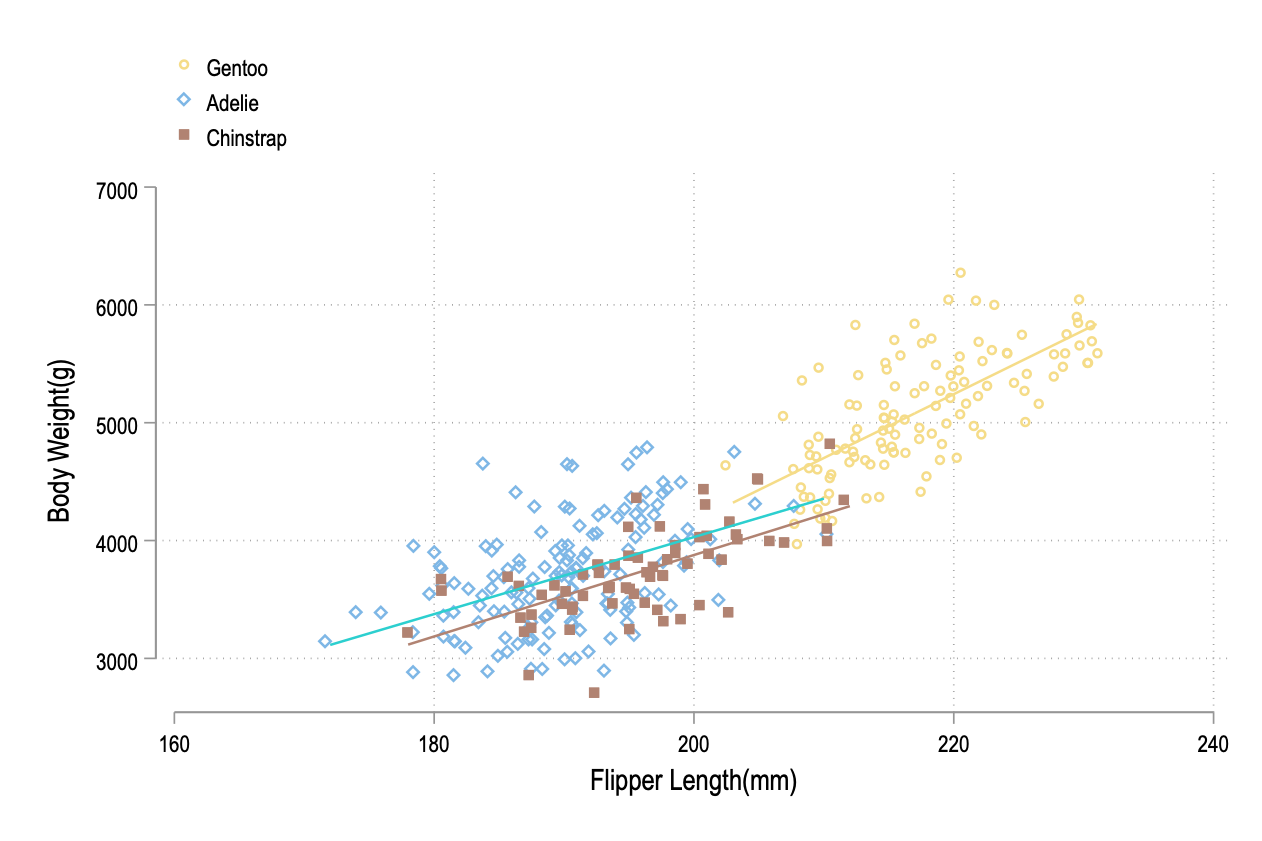
\includegraphics[width=17.53in]{penguins-manu-example} \end{center}

Whereas in R you simply need to do this

\begin{Shaded}
\begin{Highlighting}[]
\NormalTok{penguins }\OtherTok{\textless{}{-}} \FunctionTok{read\_csv}\NormalTok{(}\StringTok{"penguins.csv"}\NormalTok{)}

\NormalTok{color1 }\OtherTok{\textless{}{-}} \FunctionTok{get\_pal}\NormalTok{(}\StringTok{"Hoiho"}\NormalTok{)}

\FunctionTok{ggplot}\NormalTok{(}\AttributeTok{data =}\NormalTok{ penguins, }\FunctionTok{aes}\NormalTok{(}
  \AttributeTok{x =}\NormalTok{ flipper\_length\_mm, }\AttributeTok{y =}\NormalTok{ body\_mass\_g, }\AttributeTok{color =}\NormalTok{ species,}
  \AttributeTok{shape =}\NormalTok{ species}
\NormalTok{)) }\SpecialCharTok{+}
  \FunctionTok{geom\_point}\NormalTok{(}\AttributeTok{position =} \FunctionTok{position\_jitter}\NormalTok{(}\AttributeTok{width =} \DecValTok{0}\NormalTok{, }\AttributeTok{height =} \FloatTok{0.25}\NormalTok{, }\AttributeTok{seed =} \DecValTok{1234}\NormalTok{)) }\SpecialCharTok{+}
  \FunctionTok{geom\_smooth}\NormalTok{(}\AttributeTok{method =} \StringTok{"lm"}\NormalTok{, }\AttributeTok{se =} \ConstantTok{FALSE}\NormalTok{) }\SpecialCharTok{+}
  \FunctionTok{labs}\NormalTok{(}\AttributeTok{x =} \StringTok{"Flipper Length(mm)"}\NormalTok{, }\AttributeTok{y =} \StringTok{"Body Mass(g)"}\NormalTok{, }\AttributeTok{fill =} \StringTok{"Species of Penguins"}\NormalTok{) }\SpecialCharTok{+}
  \FunctionTok{theme\_bw}\NormalTok{() }\SpecialCharTok{+}
  \FunctionTok{scale\_color\_manual}\NormalTok{(}\AttributeTok{values =}\NormalTok{ color1) }\SpecialCharTok{+}
  \FunctionTok{scale\_x\_continuous}\NormalTok{(}\AttributeTok{breaks =}\NormalTok{ scales}\SpecialCharTok{::}\FunctionTok{pretty\_breaks}\NormalTok{(}\AttributeTok{n =} \DecValTok{10}\NormalTok{)) }\SpecialCharTok{+}
  \FunctionTok{scale\_y\_continuous}\NormalTok{(}\AttributeTok{breaks =}\NormalTok{ scales}\SpecialCharTok{::}\FunctionTok{pretty\_breaks}\NormalTok{(}\AttributeTok{n =} \DecValTok{10}\NormalTok{))}
\end{Highlighting}
\end{Shaded}

\begin{center}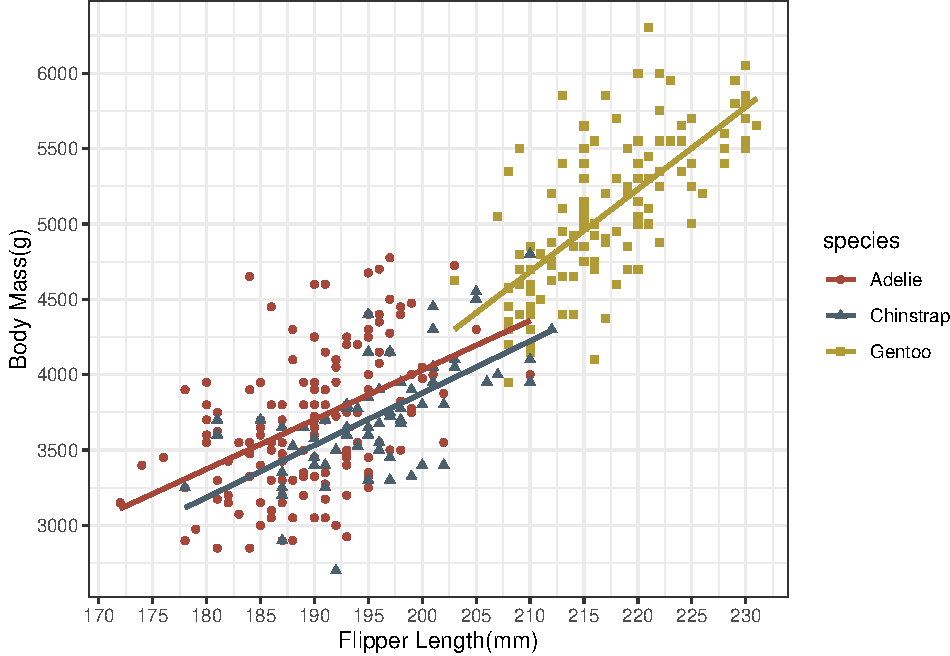
\includegraphics{R-Guide_files/figure-latex/manu-plot-1} \end{center}

Both have a sufficient amount of complexity, but this quickly becomes a
lot more complicated as you have more and more values that you need to
color in the graph. It is also hard to track because you are tricking
\texttt{Stata} by defining your own program and individually coloring
each line based on local macros and then you need to define each shape.
Additionally, the \texttt{Stata} plot has a lot of issues with
overplotting, and the hex colors don't align with the actual specified
values

The free aspect makes it incredibly attractive for many people, not
including the fact that in the data science world, \texttt{R} is one of
the most popular languages. There are lots of debates about \texttt{R}
versus \texttt{Python} versus \texttt{Julia}, but knowing any of these
three will help you learn the other because they are object-oriented
languages. \texttt{R} is not inherently better than \texttt{Stata}, but
it is not as widely used, and the fundamentals you learn in
\texttt{Stata} are not as transferable to other programming languages.

\hypertarget{getting-started}{%
\subsection{Getting Started}\label{getting-started}}

Before we start getting into R and how to use it, we should start with
workflow. It is essential to adopt what is known as project-oriented
workflow not only reproducibility, but to guard yourself against the
possibility of arson.

\begin{verbatim}
# This is bad
rm(list=ls())
set.wd("/Users/josh/Dropbox/R-Resources")

\end{verbatim}

There are lots of reasons that this bad the first point that I will
raise is a bit more technical the second is more practical for a guide
of this nature.

The first reason that you should not do this is that your workflow is
incredibly fragile and will likely have stuff in R's memory that can
cause you unknown problems. \texttt{rm(list=ls())} only removes objects
from the environment window, but all your packages remain loaded which
may cause you problems. Without a fresh \texttt{R} session you might run
into what are known as masking issues that will cause your code to
behave differently.

The more important reason is that if you have a machine at work that has
different file paths or a different operating system than a personal
machine this might also cause problems. As an example I have a laptop
and desktop that I switch between fairly often here are the directories
that this project lives on

\begin{verbatim}
setwd("/Users/Josh/Dropbox/R-Guide") ## Laptop


setwd("/Volumes/6TB Raid 10/Dropbox/R-Guide") ## Desktop
\end{verbatim}

I cannot emphasize this enough, but \texttt{R} is flexible but it only
does what it is told. For it to do something as simple as importing a
dataset it needs to know where to find that dataset. Searching for files
in \texttt{Finder} or \texttt{File\ Explorer} is effective for
\textbf{you} to find files but \textbf{not} for \texttt{R}. In
\texttt{Rstudio} you can find the dataset you need to import through
these things but that takes time each time you need to do anything. The
defaults for this approach work well enough if the data is organized
well. But that isn't often the case and will require some manipulation
when you just to import it into \texttt{R}.

Organizing things into files is the first part of making your life
easier when working with \texttt{R} or any other software language. Here
is what this guide looks like on both machines

\begin{Shaded}
\begin{Highlighting}[]
\NormalTok{knitr}\SpecialCharTok{::}\FunctionTok{include\_graphics}\NormalTok{(}\StringTok{"this\_project.png"}\NormalTok{)}
\end{Highlighting}
\end{Shaded}

\begin{center}
\includegraphics[width=28.69in]{this_project} \end{center}

For this command to work \texttt{R} needs to know where to look for
\texttt{this\_project.png}. I know which machine I am working on but
\texttt{R} does not. In \texttt{R} I cannot point and click my way to
include this picture in this document. The file path to this project is
hidden to us but it is in the same file \texttt{R-Guide} but in slightly
different locations.

When you start a new project in \texttt{R} it is like taking off in a
plane the destination is the place where that file ultimately lives. How
to get to that file is the itinerary with various stops in between. In
this case it would either be \texttt{Users}, \texttt{Josh},
\texttt{Dropbox}, and \texttt{R-Guide}. Or it would be \texttt{Volumes},
\texttt{6TB\ Raid\ 10}, \texttt{Dropbox}, and \texttt{R-Guide}. In each
flight the destination is \texttt{this\_project.png} but the route is
slightly different.

For more on project oriented workflow and why I am protecting you from
arson see this
\href{https://www.tidyverse.org/blog/2017/12/workflow-vs-script/}{post}

\hypertarget{basics}{%
\section{Basics}\label{basics}}

To start off with I think I am obligated to tell you that I am a
\texttt{tidyverse} person which has some benefits and some drawbacks. I
will not get into them but this is a future you problem. The
\texttt{tidyverse} is shorthand for a lot of packages with a similar
logic and argument structure. But not every package writer is a
tidyverse person. This will be helpful as we first learn \texttt{R}
because how people write functions differs in fairly significant ways.

\hypertarget{loading-and-installing-packages}{%
\subsection{Loading and installing
packages}\label{loading-and-installing-packages}}

When you first open \texttt{Rstudio} you have some preloaded packages.
However, I will guarantee that when you start working with \texttt{R}
more and you need to do more complex things you will have to use other
functions. The \texttt{tidyverse} is not one of these packages that is
loaded when you open \texttt{Rstudio} so if you copy and paste the code
from the knitted document it will not work. That is because \texttt{R}
does not have the instructions it needs to run those commands. In order
for it to have those directions you need to load packages with those
directions.

To do this you have to first download the package and then load the
package like this

\begin{verbatim}
install.packages("tidyverse")
library(tidyverse)
\end{verbatim}

If you want to install and load multiple packages you have to do
something like this

\begin{verbatim}
#option 1
install.packages("tidyverse")
install.packages("scales")
install.packages("Manu")

library(tidyvers)
library(scales)
library(Manu)


# option 2
install.packages(c("tidyverse","scales", "Manu"))

library(tidyvers)
library(scales)
library(Manu)



\end{verbatim}

This is what a typical \texttt{R} script looks like if you download
somebody else's code. If you want to do anything in \texttt{R} including
using our friends in the \texttt{tidyverse} you have to load the
packages in \texttt{R} or in your case since you are a brand new
\texttt{R} user you also have to download them. For the most part in
this class you will be using a lot of built in \texttt{R} functions like
\texttt{t.test}, \texttt{mean}, and friends. These are loaded in
automatically, but for the most part you are going to need add in some
friends.

\begin{verbatim}
library(tidyverse)
library(scales)
library(modelsummary)
library(kableExtra)
library(Manu)
\end{verbatim}

I use this general setup for loading and installing packages which will
appear throughout this document.

\begin{verbatim}
pacman::p_load("tidyverse", "scales", "modelsummary", "kableExtra", "Manu")


\end{verbatim}

\texttt{pacman} is a fantastic package if you are moving between
machines or sharing stuff.\footnote{Under the hood what is happening is
  that \texttt{R} is \texttt{pacman} is running \texttt{require} but it
  looks similar to the above code chunks}

I am lazy so the \texttt{library(blah)} part is a bit tedious for me,
but practically if somebody or your other machine does not have
\href{https://vincentarelbundock.github.io/modelsummary/index.html}{modelsummary}
installed or any of the other packages installed they will not have to
go through the trouble of

\begin{verbatim}
install.packages(c("all", "those", "packages", dependencies = TRUE))

library(blah)
\end{verbatim}

which is convenient but doesn't save you from some other annoying
aspects of \texttt{R}.\footnote{In order to do \texttt{pacman::p\_load}
  you have to install \texttt{pacman} via
  \texttt{install.packages("pacman")}}

\hypertarget{very-basics}{%
\subsection{Very Basics}\label{very-basics}}

So working with objects part has a few components to it so we will go
over them briefly. You will work with various kinds of things in
\texttt{R} so understanding what they are is the first step.

\hypertarget{how-we-work-with-stuff}{%
\subsubsection{How we work with stuff}\label{how-we-work-with-stuff}}

To do stuff in \texttt{R} you work off the premise that \texttt{R} is
very powerful, but with all that power you have to understand that
\texttt{R} just follows instructions without question. Lets look at this
very simple example

\begin{Shaded}
\begin{Highlighting}[]
\FunctionTok{data}\NormalTok{(mpg)}

\FunctionTok{ggplot}\NormalTok{(}\FunctionTok{aes}\NormalTok{(}\AttributeTok{x =}\NormalTok{ displ, }\AttributeTok{y =}\NormalTok{ cty)) }\SpecialCharTok{+}
  \FunctionTok{geom\_point}\NormalTok{()}
\end{Highlighting}
\end{Shaded}

\begin{verbatim}
## Error in `fortify()`:
## ! `data` must be a data frame, or other object coercible by `fortify()`, not an S3 object with class uneval.
## Did you accidentally pass `aes()` to the `data` argument?
\end{verbatim}

If you look at the environment pain we have one object \texttt{mpg} that
we are working with so \texttt{R} should know that is what we are trying
to do right? No! \texttt{R} is object oriented so you have to tell
\texttt{R} what thing you want to manipulate. There are ways around it,
but they are \textbf{\emph{strongly}} discouraged. So to get a basic
scatterplot this is what we would do.

\begin{Shaded}
\begin{Highlighting}[]
\FunctionTok{ggplot}\NormalTok{(}\AttributeTok{data =}\NormalTok{ mpg, }\FunctionTok{aes}\NormalTok{(}\AttributeTok{x =}\NormalTok{ displ, }\AttributeTok{y =}\NormalTok{ cty)) }\SpecialCharTok{+}
  \FunctionTok{geom\_point}\NormalTok{()}
\end{Highlighting}
\end{Shaded}

\begin{center}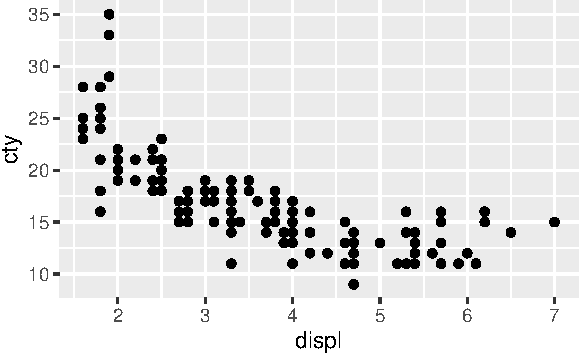
\includegraphics{R-Guide_files/figure-latex/error-fix-example-1} \end{center}

I will add a little more on this latter but for now lets just use this
as a toy example.

\hypertarget{assignment-operators}{%
\subsubsection{Assignment operators}\label{assignment-operators}}

There are three basic assignment operators \texttt{\textless{}-} is
leftward assignment and is \texttt{\textless{}} followed by \texttt{-},
\texttt{-\textgreater{}} is rightward assignment which is \texttt{-}
followed by \texttt{\textgreater{}}, and \texttt{=} is argument
assignment and leftward assignment. Most often when you look at other
people's code you will see people use \texttt{\textless{}-}. This is by
in large a convention in \texttt{R} that has been carried over from when
keyboards had \texttt{\textless{}-} on them from the mainframe computer
days. If we look at the code chunk below than you will see that all
three operators behave pretty similarly for this simple task.

\begin{Shaded}
\begin{Highlighting}[]
\NormalTok{a }\OtherTok{\textless{}{-}} \FunctionTok{c}\NormalTok{(}\DecValTok{1}\NormalTok{, }\DecValTok{3}\NormalTok{, }\DecValTok{5}\NormalTok{, }\DecValTok{6}\NormalTok{, }\DecValTok{8}\NormalTok{)}

\FunctionTok{print}\NormalTok{(a)}
\end{Highlighting}
\end{Shaded}

\begin{verbatim}
## [1] 1 3 5 6 8
\end{verbatim}

\begin{Shaded}
\begin{Highlighting}[]
\NormalTok{b }\OtherTok{\textless{}{-}} \FunctionTok{c}\NormalTok{(}\DecValTok{1}\NormalTok{, }\DecValTok{3}\NormalTok{, }\DecValTok{5}\NormalTok{, }\DecValTok{6}\NormalTok{, }\DecValTok{8}\NormalTok{)}

\FunctionTok{print}\NormalTok{(b)}
\end{Highlighting}
\end{Shaded}

\begin{verbatim}
## [1] 1 3 5 6 8
\end{verbatim}

\begin{Shaded}
\begin{Highlighting}[]
\FunctionTok{c}\NormalTok{(}\DecValTok{1}\NormalTok{, }\DecValTok{3}\NormalTok{, }\DecValTok{5}\NormalTok{, }\DecValTok{6}\NormalTok{, }\DecValTok{8}\NormalTok{) }\OtherTok{{-}\textgreater{}}\NormalTok{ d}

\FunctionTok{print}\NormalTok{(d)}
\end{Highlighting}
\end{Shaded}

\begin{verbatim}
## [1] 1 3 5 6 8
\end{verbatim}

I am what most would call lazy so I prefer \texttt{=} over
\texttt{\textless{}-} for convenience sake. However, there are valid
reasons to prefer one over the other. There are various arguments for or
against both. The difference real comes down to preference. \footnote{\href{https://github.com/Robinlovelace/geocompr/issues/319\#issuecomment-427376764}{this
  is a good top level summary} and
  \href{https://www.separatinghyperplanes.com/2018/02/why-you-should-use-and-never.html}{this
  which is a more in depth coverage}}

\hypertarget{types-of-stuff}{%
\subsubsection{Types of Stuff}\label{types-of-stuff}}

We have a few basic kinds of classes in \texttt{R}

\begin{itemize}
\tightlist
\item
  character: (``a'', ``swc'')
\item
  numeric(real or decimal): (2, 15.5)
\item
  integer: 2, -2, 7
\item
  logical: \texttt{TRUE}, \texttt{FALSE}
\item
  date: 11-24-2021
\end{itemize}

Different arguments take different classes of variables. Sometimes you
need to coerce variables to be of a kind of class, but these are what
you are going to work with most of the time.

\hypertarget{vectors}{%
\subsubsection{Vectors}\label{vectors}}

The first thing we work with are vectors which are the most basic that
can \emph{be} various \texttt{classes}.

\begin{Shaded}
\begin{Highlighting}[]
\NormalTok{x }\OtherTok{\textless{}{-}} \FunctionTok{c}\NormalTok{(}\DecValTok{1}\NormalTok{, }\DecValTok{3}\NormalTok{, }\DecValTok{5}\NormalTok{, }\DecValTok{6}\NormalTok{, }\DecValTok{8}\NormalTok{)}

\NormalTok{x}
\end{Highlighting}
\end{Shaded}

\begin{verbatim}
## [1] 1 3 5 6 8
\end{verbatim}

\begin{Shaded}
\begin{Highlighting}[]
\FunctionTok{class}\NormalTok{(x)}
\end{Highlighting}
\end{Shaded}

\begin{verbatim}
## [1] "numeric"
\end{verbatim}

\begin{Shaded}
\begin{Highlighting}[]
\NormalTok{z }\OtherTok{\textless{}{-}} \FunctionTok{c}\NormalTok{(}\StringTok{"a"}\NormalTok{, }\StringTok{"b"}\NormalTok{, }\StringTok{"c"}\NormalTok{, }\StringTok{"d"}\NormalTok{, }\StringTok{"e"}\NormalTok{)}

\NormalTok{z}
\end{Highlighting}
\end{Shaded}

\begin{verbatim}
## [1] "a" "b" "c" "d" "e"
\end{verbatim}

\begin{Shaded}
\begin{Highlighting}[]
\FunctionTok{class}\NormalTok{(z)}
\end{Highlighting}
\end{Shaded}

\begin{verbatim}
## [1] "character"
\end{verbatim}

So to break down what happened here we made a vector \texttt{x} by doing
\texttt{x\ =\ c(1,\ 3,\ 5,\ 6,\ 8)} where \texttt{c} means concatenate
which basically just means this stuff goes together. \texttt{class}
returns what type of vector it is which is really useful when you are
trying to figure out what is going on with your code. For the most part
a vector is going to be a column in your dataset. This is an indpendent
variable, a dependent variable, or a confounding variable that we can
easily manipulate.

Consider the example below where we just multiply \texttt{x} by 2. If we
just want to multiply it by two that is fine. But if we want to work
with \texttt{x*2} we have to assign it to a \textbf{new} object.

\begin{Shaded}
\begin{Highlighting}[]
\NormalTok{x }\SpecialCharTok{*} \DecValTok{2}
\end{Highlighting}
\end{Shaded}

\begin{verbatim}
## [1]  2  6 10 12 16
\end{verbatim}

\begin{Shaded}
\begin{Highlighting}[]
\NormalTok{x2 }\OtherTok{\textless{}{-}}\NormalTok{ x }\SpecialCharTok{*} \DecValTok{2}

\NormalTok{x2}
\end{Highlighting}
\end{Shaded}

\begin{verbatim}
## [1]  2  6 10 12 16
\end{verbatim}

We can get basic descriptive statistics of both vectors by doing

\begin{Shaded}
\begin{Highlighting}[]
\FunctionTok{summary}\NormalTok{(x)}
\end{Highlighting}
\end{Shaded}

\begin{verbatim}
##    Min. 1st Qu.  Median    Mean 3rd Qu.    Max. 
##     1.0     3.0     5.0     4.6     6.0     8.0
\end{verbatim}

\hypertarget{lists}{%
\subsubsection{Lists}\label{lists}}

a \texttt{list} is something we will work with a lot that can
\emph{contain} various classes

\begin{Shaded}
\begin{Highlighting}[]
\NormalTok{list1 }\OtherTok{\textless{}{-}} \FunctionTok{list}\NormalTok{(}\DecValTok{1}\NormalTok{, }\DecValTok{2}\NormalTok{, }\DecValTok{3}\NormalTok{)}

\NormalTok{list2 }\OtherTok{\textless{}{-}} \FunctionTok{list}\NormalTok{(}\StringTok{"Sun"}\NormalTok{, }\StringTok{"Mon"}\NormalTok{, }\StringTok{"Tue"}\NormalTok{)}

\NormalTok{list3 }\OtherTok{\textless{}{-}} \FunctionTok{c}\NormalTok{(list1, list2)}

\FunctionTok{print}\NormalTok{(list3)}
\end{Highlighting}
\end{Shaded}

\begin{verbatim}
## [[1]]
## [1] 1
## 
## [[2]]
## [1] 2
## 
## [[3]]
## [1] 3
## 
## [[4]]
## [1] "Sun"
## 
## [[5]]
## [1] "Mon"
## 
## [[6]]
## [1] "Tue"
\end{verbatim}

\hypertarget{matrices}{%
\subsection{Matrices}\label{matrices}}

You can think of matrices as a dataset so our \texttt{mpg} dataset is a
matrix. If we do this

\begin{Shaded}
\begin{Highlighting}[]
\NormalTok{y }\OtherTok{\textless{}{-}} \FunctionTok{cbind}\NormalTok{(a, z)}

\NormalTok{y}
\end{Highlighting}
\end{Shaded}

\begin{verbatim}
##      a   z  
## [1,] "1" "a"
## [2,] "3" "b"
## [3,] "5" "c"
## [4,] "6" "d"
## [5,] "8" "e"
\end{verbatim}

now we have a matrix of our vectors that we made earlier. A matrix is
just two or more vectors combined together. This should be intuitive if
you have ever run into matrix algebra.

\hypertarget{manipulating-data}{%
\section{Manipulating data}\label{manipulating-data}}

To add a huge caveat. If you are moving over from Excel or Stata you
have the option of manipulating data through a drop down or just
recoding the variable either through \texttt{edit} in Stata or just
changing the number in the cell.

However whenever possible you want to do this through code. It is
transparent and reproducible which lets other people learn and you have
it forever. Practically it is also quicker in many cases becasue the
computer can do it quicker and more accurately if it is given the right
instructions. There are a bunch of ways to do it so we will separate it
into a few ways.

\hypertarget{dplyr}{%
\subsection{\texorpdfstring{\texttt{dplyr}}{dplyr}}\label{dplyr}}

\texttt{dplyr} is a great package that I use all the time to clean data.
But you need to get the basic functions right. Cleaning data is what you
will spend the most time on.

\hypertarget{boolean-operators}{%
\subsubsection{Boolean Operators}\label{boolean-operators}}

So before we start working with our friends \texttt{select},
\texttt{filter}, \texttt{mutate}, and \texttt{summarize} we should start
with what Boolean operators are because they are how we get what we want
in working with \texttt{dplyr}. So lets start by working with the the
\texttt{starwars} dataset.

\begin{Shaded}
\begin{Highlighting}[]
\FunctionTok{data}\NormalTok{(}\StringTok{"starwars"}\NormalTok{)}
\FunctionTok{head}\NormalTok{(starwars)}
\end{Highlighting}
\end{Shaded}

\begin{verbatim}
## # A tibble: 6 x 14
##   name      height  mass hair_color skin_color eye_color birth_year sex   gender
##   <chr>      <int> <dbl> <chr>      <chr>      <chr>          <dbl> <chr> <chr> 
## 1 Luke Sky~    172    77 blond      fair       blue            19   male  mascu~
## 2 C-3PO        167    75 <NA>       gold       yellow         112   none  mascu~
## 3 R2-D2         96    32 <NA>       white, bl~ red             33   none  mascu~
## 4 Darth Va~    202   136 none       white      yellow          41.9 male  mascu~
## 5 Leia Org~    150    49 brown      light      brown           19   fema~ femin~
## 6 Owen Lars    178   120 brown, gr~ light      blue            52   male  mascu~
## # ... with 5 more variables: homeworld <chr>, species <chr>, films <list>,
## #   vehicles <list>, starships <list>
\end{verbatim}

So we have our data in now lets try manipulate the data where we only
care about droids. So lets do that through our friend \texttt{filter}

\begin{Shaded}
\begin{Highlighting}[]
\FunctionTok{filter}\NormalTok{(starwars, }\AttributeTok{species =} \StringTok{"Droid"}\NormalTok{)}
\end{Highlighting}
\end{Shaded}

\begin{verbatim}
## Error in `filter()`:
## ! We detected a named input.
## i This usually means that you've used `=` instead of `==`.
## i Did you mean `species == "Droid"`?
\end{verbatim}

As you can see \texttt{filter} throws an error because we aren't using
our Boolean operators. These are your boolean operators

\begin{itemize}
\tightlist
\item
  \texttt{==} is equal to
\item
  \texttt{!} is equivalent to not
\item
  \texttt{\textbar{}} is equivalent to or
\item
  \texttt{\textgreater{}} is greater than
\item
  \texttt{\textless{}} is less than
\item
  \texttt{!=} is not equal to
\item
  \texttt{\textgreater{}=} is greater than or equal to
\item
  \texttt{\textless{}=} is less than or equal to
\item
  \texttt{\&} is and
\end{itemize}

\hypertarget{filter}{%
\subsubsection{\texorpdfstring{\texttt{filter}}{filter}}\label{filter}}

Lets combine what we just learned

\begin{Shaded}
\begin{Highlighting}[]
\FunctionTok{filter}\NormalTok{(mpg, manufacturer }\SpecialCharTok{==} \StringTok{"audi"}\NormalTok{)}
\end{Highlighting}
\end{Shaded}

\begin{verbatim}
## # A tibble: 18 x 11
##    manufacturer model      displ  year   cyl trans drv     cty   hwy fl    class
##    <chr>        <chr>      <dbl> <int> <int> <chr> <chr> <int> <int> <chr> <chr>
##  1 audi         a4           1.8  1999     4 auto~ f        18    29 p     comp~
##  2 audi         a4           1.8  1999     4 manu~ f        21    29 p     comp~
##  3 audi         a4           2    2008     4 manu~ f        20    31 p     comp~
##  4 audi         a4           2    2008     4 auto~ f        21    30 p     comp~
##  5 audi         a4           2.8  1999     6 auto~ f        16    26 p     comp~
##  6 audi         a4           2.8  1999     6 manu~ f        18    26 p     comp~
##  7 audi         a4           3.1  2008     6 auto~ f        18    27 p     comp~
##  8 audi         a4 quattro   1.8  1999     4 manu~ 4        18    26 p     comp~
##  9 audi         a4 quattro   1.8  1999     4 auto~ 4        16    25 p     comp~
## 10 audi         a4 quattro   2    2008     4 manu~ 4        20    28 p     comp~
## 11 audi         a4 quattro   2    2008     4 auto~ 4        19    27 p     comp~
## 12 audi         a4 quattro   2.8  1999     6 auto~ 4        15    25 p     comp~
## 13 audi         a4 quattro   2.8  1999     6 manu~ 4        17    25 p     comp~
## 14 audi         a4 quattro   3.1  2008     6 auto~ 4        17    25 p     comp~
## 15 audi         a4 quattro   3.1  2008     6 manu~ 4        15    25 p     comp~
## 16 audi         a6 quattro   2.8  1999     6 auto~ 4        15    24 p     mids~
## 17 audi         a6 quattro   3.1  2008     6 auto~ 4        17    25 p     mids~
## 18 audi         a6 quattro   4.2  2008     8 auto~ 4        16    23 p     mids~
\end{verbatim}

\begin{Shaded}
\begin{Highlighting}[]
\FunctionTok{filter}\NormalTok{(starwars, homeworld }\SpecialCharTok{==} \StringTok{"Naboo"}\NormalTok{)}
\end{Highlighting}
\end{Shaded}

\begin{verbatim}
## # A tibble: 11 x 14
##    name     height  mass hair_color skin_color eye_color birth_year sex   gender
##    <chr>     <int> <dbl> <chr>      <chr>      <chr>          <dbl> <chr> <chr> 
##  1 R2-D2        96    32 <NA>       white, bl~ red               33 none  mascu~
##  2 Palpati~    170    75 grey       pale       yellow            82 male  mascu~
##  3 Jar Jar~    196    66 none       orange     orange            52 male  mascu~
##  4 Roos Ta~    224    82 none       grey       orange            NA male  mascu~
##  5 Rugor N~    206    NA none       green      orange            NA male  mascu~
##  6 Ric Olié    183    NA brown      fair       blue              NA <NA>  <NA>  
##  7 Quarsh ~    183    NA black      dark       brown             62 <NA>  <NA>  
##  8 Gregar ~    185    85 black      dark       brown             NA male  mascu~
##  9 Cordé       157    NA brown      light      brown             NA fema~ femin~
## 10 Dormé       165    NA brown      light      brown             NA fema~ femin~
## 11 Padmé A~    165    45 brown      light      brown             46 fema~ femin~
## # ... with 5 more variables: homeworld <chr>, species <chr>, films <list>,
## #   vehicles <list>, starships <list>
\end{verbatim}

\begin{Shaded}
\begin{Highlighting}[]
\FunctionTok{filter}\NormalTok{(starwars, homeworld }\SpecialCharTok{!=} \StringTok{"Naboo"}\NormalTok{)}
\end{Highlighting}
\end{Shaded}

\begin{verbatim}
## # A tibble: 66 x 14
##    name     height  mass hair_color skin_color eye_color birth_year sex   gender
##    <chr>     <int> <dbl> <chr>      <chr>      <chr>          <dbl> <chr> <chr> 
##  1 Luke Sk~    172    77 blond      fair       blue            19   male  mascu~
##  2 C-3PO       167    75 <NA>       gold       yellow         112   none  mascu~
##  3 Darth V~    202   136 none       white      yellow          41.9 male  mascu~
##  4 Leia Or~    150    49 brown      light      brown           19   fema~ femin~
##  5 Owen La~    178   120 brown, gr~ light      blue            52   male  mascu~
##  6 Beru Wh~    165    75 brown      light      blue            47   fema~ femin~
##  7 R5-D4        97    32 <NA>       white, red red             NA   none  mascu~
##  8 Biggs D~    183    84 black      light      brown           24   male  mascu~
##  9 Obi-Wan~    182    77 auburn, w~ fair       blue-gray       57   male  mascu~
## 10 Anakin ~    188    84 blond      fair       blue            41.9 male  mascu~
## # ... with 56 more rows, and 5 more variables: homeworld <chr>, species <chr>,
## #   films <list>, vehicles <list>, starships <list>
\end{verbatim}

What we are doing here is just creating a dataset with just stuff made
by audi, just things from Naboo, and where everything is not from Naboo.
But, this isn't actually going to do anything yet. If you want this to
become a real dataset you need to create a new object. So lets just take
the starwars data and create a naboo object.

\begin{Shaded}
\begin{Highlighting}[]
\NormalTok{naboo }\OtherTok{\textless{}{-}} \FunctionTok{filter}\NormalTok{(starwars, homeworld }\SpecialCharTok{==} \StringTok{"Naboo"}\NormalTok{)}
\end{Highlighting}
\end{Shaded}

You can also make an object combining boolean operators like this

\begin{Shaded}
\begin{Highlighting}[]
\NormalTok{naboo2 }\OtherTok{\textless{}{-}} \FunctionTok{filter}\NormalTok{(starwars, homeworld }\SpecialCharTok{==} \StringTok{"Naboo"} \SpecialCharTok{\&}\NormalTok{ species }\SpecialCharTok{==} \StringTok{"Human"}\NormalTok{)}
\end{Highlighting}
\end{Shaded}

Now we have all the characters that are from Naboo and are human!

When working with things in \texttt{R} stray commas and spelling will
lead to head aches. here is an example that would not throw an error but
will create a dataframe with zero observations. Naboo exists as a value
of homeworld but naboo does not.

\begin{Shaded}
\begin{Highlighting}[]
\NormalTok{naboo }\OtherTok{\textless{}{-}} \FunctionTok{filter}\NormalTok{(starwars, homeworld }\SpecialCharTok{==} \StringTok{"naboo"}\NormalTok{)}

\NormalTok{naboo }\OtherTok{\textless{}{-}} \FunctionTok{filter}\NormalTok{(starwars, homeworld }\SpecialCharTok{==} \StringTok{"Naboo"}\NormalTok{, )}
\end{Highlighting}
\end{Shaded}

\hypertarget{mutate}{%
\subsubsection{\texorpdfstring{\texttt{mutate}}{mutate}}\label{mutate}}

\texttt{mutate} is how we create new columns in our dataset. So lets
take our starwars dataset and create a new column which is an indicator
variable for whether or not a character is a human or not

\begin{Shaded}
\begin{Highlighting}[]
\NormalTok{starwars\_human }\OtherTok{\textless{}{-}}\NormalTok{ starwars }\SpecialCharTok{\%\textgreater{}\%}
  \FunctionTok{mutate}\NormalTok{(}\AttributeTok{human =} \FunctionTok{ifelse}\NormalTok{(species }\SpecialCharTok{==} \StringTok{"Human"}\NormalTok{, }\ConstantTok{TRUE}\NormalTok{, }\ConstantTok{FALSE}\NormalTok{)) }\SpecialCharTok{\%\textgreater{}\%}
  \FunctionTok{select}\NormalTok{(human, name)}

\FunctionTok{head}\NormalTok{(starwars\_human)}
\end{Highlighting}
\end{Shaded}

\begin{verbatim}
## # A tibble: 6 x 2
##   human name          
##   <lgl> <chr>         
## 1 TRUE  Luke Skywalker
## 2 FALSE C-3PO         
## 3 FALSE R2-D2         
## 4 TRUE  Darth Vader   
## 5 TRUE  Leia Organa   
## 6 TRUE  Owen Lars
\end{verbatim}

Here we are doing a little bit more stuff than we have covered. So lets
walk through it. We made a new variable called \texttt{human} if
\texttt{species} takes the value of human. \texttt{R} recognizes
\texttt{TRUE} and \texttt{FALSE} but you can also sub in \texttt{1} and
\texttt{0} and \texttt{R} will treat them virtually the same. We also
introduced your best friend \texttt{\%\textgreater{}\%} which is
technically called a pipe. However, you should read it as \textbf{and
then}. The easiest way to think of the pipe when working through stuff
is this way from
\href{https://twitter.com/andrewheiss/status/1359583543509348356?lang=en}{Andrew
Heiss} using your morning routine.

\begin{verbatim}
me %>% 
wake_up(time = "8.00am") %>% 
get_out_of_bed(side = "correct") %>% 
get_dressed(pants = "TRUE", shirt = "TRUE") %>% 
leave_house(car = TRUE, bike = FALSE, MARTA = FALSE) %>% 
am_late(traffic = TRUE)
\end{verbatim}

Our friend mutate can do a lot. So lets make a column in our dataset
where we see how old a character is in dog years with a description so
other people know what is going on!

\begin{Shaded}
\begin{Highlighting}[]
\NormalTok{starwars }\SpecialCharTok{\%\textgreater{}\%}
  \FunctionTok{filter}\NormalTok{(}\SpecialCharTok{!}\FunctionTok{is.na}\NormalTok{(birth\_year)) }\SpecialCharTok{\%\textgreater{}\%}
  \FunctionTok{select}\NormalTok{(name, birth\_year) }\SpecialCharTok{\%\textgreater{}\%}
  \FunctionTok{mutate}\NormalTok{(}\AttributeTok{dog\_years =}\NormalTok{ birth\_year }\SpecialCharTok{*} \DecValTok{7}\NormalTok{) }\SpecialCharTok{\%\textgreater{}\%}
  \FunctionTok{mutate}\NormalTok{(}\AttributeTok{comment =} \FunctionTok{paste0}\NormalTok{(name, }\StringTok{" is "}\NormalTok{, dog\_years, }\StringTok{" in dog years."}\NormalTok{))}
\end{Highlighting}
\end{Shaded}

\begin{verbatim}
## # A tibble: 43 x 4
##    name               birth_year dog_years comment                              
##    <chr>                   <dbl>     <dbl> <chr>                                
##  1 Luke Skywalker           19        133  Luke Skywalker is 133 in dog years.  
##  2 C-3PO                   112        784  C-3PO is 784 in dog years.           
##  3 R2-D2                    33        231  R2-D2 is 231 in dog years.           
##  4 Darth Vader              41.9      293. Darth Vader is 293.3 in dog years.   
##  5 Leia Organa              19        133  Leia Organa is 133 in dog years.     
##  6 Owen Lars                52        364  Owen Lars is 364 in dog years.       
##  7 Beru Whitesun lars       47        329  Beru Whitesun lars is 329 in dog yea~
##  8 Biggs Darklighter        24        168  Biggs Darklighter is 168 in dog year~
##  9 Obi-Wan Kenobi           57        399  Obi-Wan Kenobi is 399 in dog years.  
## 10 Anakin Skywalker         41.9      293. Anakin Skywalker is 293.3 in dog yea~
## # ... with 33 more rows
\end{verbatim}

You can make this code more concise because \texttt{mutate} is order
aware this will do the exact same thing.

\begin{Shaded}
\begin{Highlighting}[]
\NormalTok{starwars }\SpecialCharTok{\%\textgreater{}\%}
  \FunctionTok{filter}\NormalTok{(}\SpecialCharTok{!}\FunctionTok{is.na}\NormalTok{(birth\_year)) }\SpecialCharTok{\%\textgreater{}\%}
  \FunctionTok{select}\NormalTok{(name, birth\_year) }\SpecialCharTok{\%\textgreater{}\%}
  \FunctionTok{mutate}\NormalTok{(}
    \AttributeTok{dog\_years =}\NormalTok{ birth\_year }\SpecialCharTok{*} \DecValTok{7}\NormalTok{,}
    \AttributeTok{comment =} \FunctionTok{paste0}\NormalTok{(name, }\StringTok{" is "}\NormalTok{, dog\_years, }\StringTok{" in dog years."}\NormalTok{)}
\NormalTok{  )}
\end{Highlighting}
\end{Shaded}

\begin{verbatim}
## # A tibble: 43 x 4
##    name               birth_year dog_years comment                              
##    <chr>                   <dbl>     <dbl> <chr>                                
##  1 Luke Skywalker           19        133  Luke Skywalker is 133 in dog years.  
##  2 C-3PO                   112        784  C-3PO is 784 in dog years.           
##  3 R2-D2                    33        231  R2-D2 is 231 in dog years.           
##  4 Darth Vader              41.9      293. Darth Vader is 293.3 in dog years.   
##  5 Leia Organa              19        133  Leia Organa is 133 in dog years.     
##  6 Owen Lars                52        364  Owen Lars is 364 in dog years.       
##  7 Beru Whitesun lars       47        329  Beru Whitesun lars is 329 in dog yea~
##  8 Biggs Darklighter        24        168  Biggs Darklighter is 168 in dog year~
##  9 Obi-Wan Kenobi           57        399  Obi-Wan Kenobi is 399 in dog years.  
## 10 Anakin Skywalker         41.9      293. Anakin Skywalker is 293.3 in dog yea~
## # ... with 33 more rows
\end{verbatim}

Data cleaning is the vast majority of what you will be doing if you open
up a dataset. You will spend a lot of mental energy on learning how the
stats behind what happens when you estimate models. However, whether you
run something as simple as

\begin{verbatim}
lm(y ~ x1 + x2 + x3, data = blah)
\end{verbatim}

or are making graphs. Data cleaning is a skill that you have to practice
in order to make any claims about your data. \#\#\# \texttt{select}

Now lets move on to our friend \texttt{select}. \texttt{Select} will
literally just select columns from your object that you specify. So lets
take our object \texttt{starwars\_humnan} and then go really extreme and
just take the \texttt{human} column and our name column.

\begin{Shaded}
\begin{Highlighting}[]
\NormalTok{extreme }\OtherTok{\textless{}{-}}\NormalTok{ starwars\_human }\SpecialCharTok{\%\textgreater{}\%}
  \FunctionTok{select}\NormalTok{(human, name)}

\FunctionTok{head}\NormalTok{(extreme)}
\end{Highlighting}
\end{Shaded}

\begin{verbatim}
## # A tibble: 6 x 2
##   human name          
##   <lgl> <chr>         
## 1 TRUE  Luke Skywalker
## 2 FALSE C-3PO         
## 3 FALSE R2-D2         
## 4 TRUE  Darth Vader   
## 5 TRUE  Leia Organa   
## 6 TRUE  Owen Lars
\end{verbatim}

\hypertarget{group_by-and-summarize}{%
\subsubsection{\texorpdfstring{\texttt{group\_by} and
\texttt{summarize}}{group\_by and summarize}}\label{group_by-and-summarize}}

I tend to use these two commands together because they are pretty well
matched. \texttt{group\_by} collapses data to single row by a column or
columns in our dataset. Think of this as collapsing our data to your
unit of analysis. Like country or if you have panel data where we
observing multiple countries over multiple years we can use
\texttt{group\_by} to look at \texttt{country\ and\ year}. To see a
simple example lets load in data that tracks flights out of New York
City.

\begin{Shaded}
\begin{Highlighting}[]
\NormalTok{pacman}\SpecialCharTok{::}\FunctionTok{p\_load}\NormalTok{(}\StringTok{"nycflights13"}\NormalTok{)}

\FunctionTok{data}\NormalTok{(flights)}
\end{Highlighting}
\end{Shaded}

Imagine that we want to explore the relationship between the distance
and average delay for each location. Using what you know about dplyr,
you might write code like this with pipes. We should also remove missing
values with \texttt{na.rm\ =\ TRUE}.

\begin{Shaded}
\begin{Highlighting}[]
\NormalTok{delays }\OtherTok{\textless{}{-}}\NormalTok{ flights }\SpecialCharTok{\%\textgreater{}\%}
  \FunctionTok{group\_by}\NormalTok{(dest) }\SpecialCharTok{\%\textgreater{}\%}
  \FunctionTok{summarise}\NormalTok{(}
    \AttributeTok{count =} \FunctionTok{n}\NormalTok{(),}
    \AttributeTok{dist =} \FunctionTok{mean}\NormalTok{(distance, }\AttributeTok{na.rm =} \ConstantTok{TRUE}\NormalTok{),}
    \AttributeTok{delay =} \FunctionTok{mean}\NormalTok{(arr\_delay, }\AttributeTok{na.rm =} \ConstantTok{TRUE}\NormalTok{)}
\NormalTok{  ) }\SpecialCharTok{\%\textgreater{}\%}
  \FunctionTok{filter}\NormalTok{(count }\SpecialCharTok{\textgreater{}} \DecValTok{20}\NormalTok{, dest }\SpecialCharTok{!=} \StringTok{"HNL"}\NormalTok{)}
\end{Highlighting}
\end{Shaded}

Then lets plot the data the data for fun!

\begin{Shaded}
\begin{Highlighting}[]
\FunctionTok{ggplot}\NormalTok{(}\AttributeTok{data =}\NormalTok{ delays, }\AttributeTok{mapping =} \FunctionTok{aes}\NormalTok{(}\AttributeTok{x =}\NormalTok{ dist, }\AttributeTok{y =}\NormalTok{ delay)) }\SpecialCharTok{+}
  \FunctionTok{geom\_point}\NormalTok{(}\FunctionTok{aes}\NormalTok{(}\AttributeTok{size =}\NormalTok{ count), }\AttributeTok{alpha =} \DecValTok{1} \SpecialCharTok{/} \DecValTok{3}\NormalTok{) }\SpecialCharTok{+}
  \FunctionTok{geom\_smooth}\NormalTok{(}\AttributeTok{se =} \ConstantTok{FALSE}\NormalTok{)}
\end{Highlighting}
\end{Shaded}

\begin{center}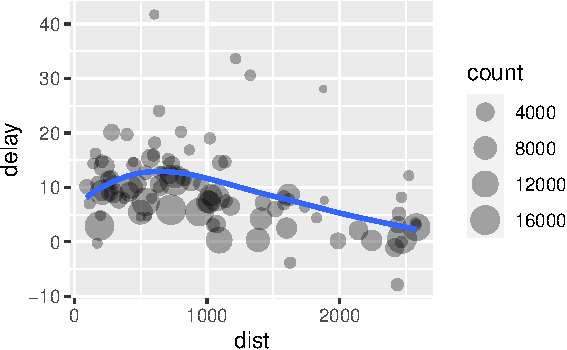
\includegraphics{R-Guide_files/figure-latex/unnamed-chunk-9-1} \end{center}

What if we forgot our friend \texttt{group\_by}? Well unfortunately
\texttt{filter} does not work in this case so we had to delete that. Now
what happened is we are getting a single value for each of the variables
we initially wanted, but it is not entirely helpful.

\begin{Shaded}
\begin{Highlighting}[]
\NormalTok{delay }\OtherTok{\textless{}{-}}\NormalTok{ flights }\SpecialCharTok{\%\textgreater{}\%}
  \FunctionTok{summarise}\NormalTok{(}
    \AttributeTok{count =} \FunctionTok{n}\NormalTok{(),}
    \AttributeTok{dist =} \FunctionTok{mean}\NormalTok{(distance, }\AttributeTok{na.rm =} \ConstantTok{TRUE}\NormalTok{),}
    \AttributeTok{delay =} \FunctionTok{mean}\NormalTok{(arr\_delay, }\AttributeTok{na.rm =} \ConstantTok{TRUE}\NormalTok{)}
\NormalTok{  )}
\end{Highlighting}
\end{Shaded}

Then lets plot the data!

\begin{Shaded}
\begin{Highlighting}[]
\FunctionTok{ggplot}\NormalTok{(}\AttributeTok{data =}\NormalTok{ delay, }\AttributeTok{mapping =} \FunctionTok{aes}\NormalTok{(}\AttributeTok{x =}\NormalTok{ dist, }\AttributeTok{y =}\NormalTok{ delay)) }\SpecialCharTok{+}
  \FunctionTok{geom\_point}\NormalTok{(}\FunctionTok{aes}\NormalTok{(}\AttributeTok{size =}\NormalTok{ count), }\AttributeTok{alpha =} \DecValTok{1} \SpecialCharTok{/} \DecValTok{3}\NormalTok{) }\SpecialCharTok{+}
  \FunctionTok{geom\_smooth}\NormalTok{(}\AttributeTok{se =} \ConstantTok{FALSE}\NormalTok{)}
\end{Highlighting}
\end{Shaded}

\begin{center}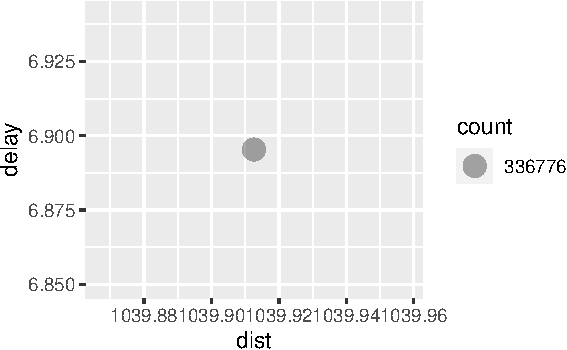
\includegraphics{R-Guide_files/figure-latex/unnamed-chunk-11-1} \end{center}

\hypertarget{data-vizsualization}{%
\section{Data Vizsualization}\label{data-vizsualization}}

We will cover this more in depth but the skill that will carry help you
stand out or help you understand what is going on is being able to
present your findings and data graphically. People are good at seeing
patterns in stuff so it will be helpful to get a basic grasp of the most
popular \texttt{tidyverse} friend \texttt{ggplot}. Lets some toy data
about penguins to go through this example and load in a package named
\texttt{patchwork} and \texttt{ggthemes}.

\begin{Shaded}
\begin{Highlighting}[]
\NormalTok{pacman}\SpecialCharTok{::}\FunctionTok{p\_load}\NormalTok{(}\StringTok{"patchwork"}\NormalTok{, }\StringTok{"ggthemes"}\NormalTok{)}


\NormalTok{penguins }\OtherTok{\textless{}{-}} \FunctionTok{read\_csv}\NormalTok{(}\StringTok{"penguins.csv"}\NormalTok{)}
\end{Highlighting}
\end{Shaded}

The function we are going to be working with is \texttt{ggplot} there
are a lot of components to it and it is a little overwhelming at first.
But this is the basic logic of \texttt{ggplot}

\begin{itemize}
\tightlist
\item
  \texttt{data} tells \texttt{R} what data we are using for this plot.
\item
  \texttt{aes} tells \texttt{R} what columns in the dataset we want
  graphed
\item
  \texttt{geom\_blah} tells \texttt{R} what kind of plot we want.
\end{itemize}

As an example in \texttt{Stata} it is
\texttt{tw\ scatter\ varlist,\ options} to create a scatter plot. We
will see how that differs.

Here is a basic scatter plot in \texttt{ggplot}

\begin{Shaded}
\begin{Highlighting}[]
\FunctionTok{ggplot}\NormalTok{(}\AttributeTok{data =}\NormalTok{ penguins) }\SpecialCharTok{+}
  \FunctionTok{geom\_point}\NormalTok{(}\FunctionTok{aes}\NormalTok{(}\AttributeTok{x =}\NormalTok{ flipper\_length\_mm, }\AttributeTok{y =}\NormalTok{ body\_mass\_g))}
\end{Highlighting}
\end{Shaded}

\begin{center}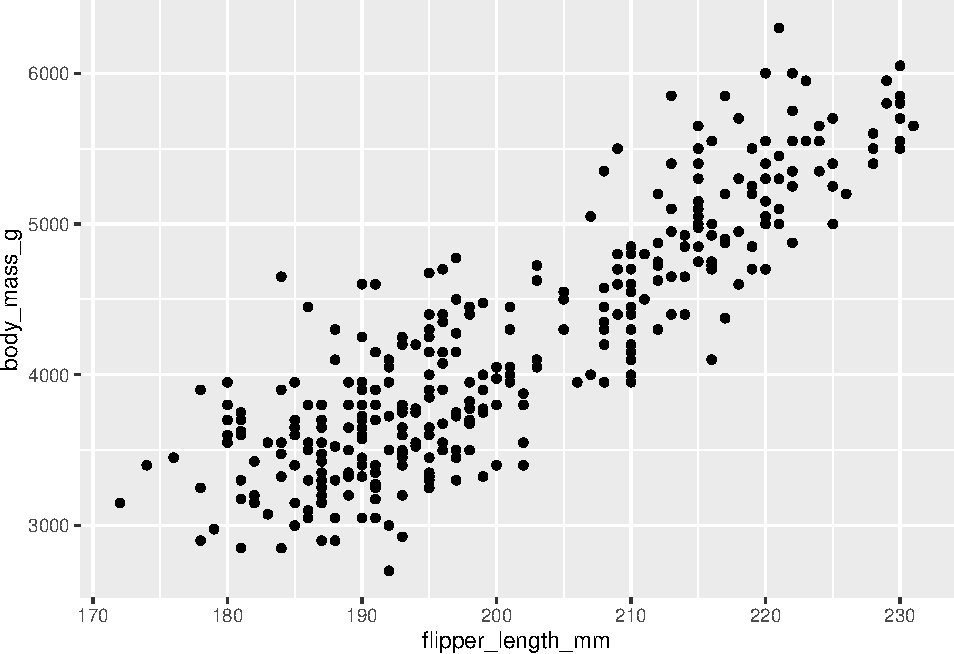
\includegraphics{R-Guide_files/figure-latex/scatter-basic-1} \end{center}

Notice that in \texttt{aes} we told \texttt{R} what columns to use for
our \texttt{x} and \texttt{y} axis. Unlike \texttt{Stata} or
\texttt{SAS} we have to tell \texttt{R} what object to use. Whereas in
Stata you would do this

\begin{verbatim}
tw scatter body_mass_g flipper_length_mm
\end{verbatim}

\texttt{R} has a lot of solutions to the same problem This is usually
how I graph stuff. \href{https://r4ds.had.co.nz/index.html}{\texttt{R}
for Datascience} covers this better than I could. Since this is an intro
we will side step style guides and just work with what I do.

\begin{Shaded}
\begin{Highlighting}[]
\FunctionTok{ggplot}\NormalTok{(penguins, }\FunctionTok{aes}\NormalTok{(}\AttributeTok{x =}\NormalTok{ flipper\_length\_mm, }\AttributeTok{y =}\NormalTok{ body\_mass\_g)) }\SpecialCharTok{+}
  \FunctionTok{geom\_point}\NormalTok{()}
\end{Highlighting}
\end{Shaded}

\begin{center}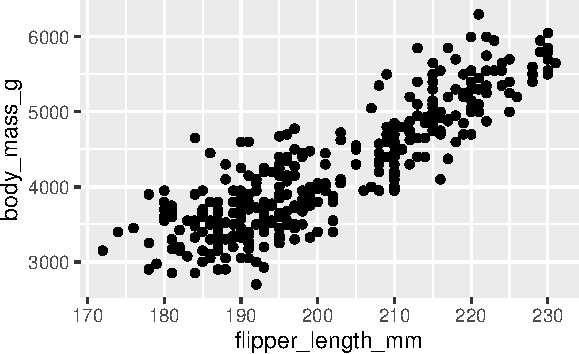
\includegraphics{R-Guide_files/figure-latex/scatter-basic-global-1} \end{center}

Like \texttt{Stata} you need to add stuff to customize plot when you add
stuff instead of \texttt{,options} you use \texttt{+} and then add
stuff. Here is an example of things you can add, but this is only the
tip of the iceberg.

\begin{Shaded}
\begin{Highlighting}[]
\FunctionTok{ggplot}\NormalTok{(penguins, }\FunctionTok{aes}\NormalTok{(}\AttributeTok{x =}\NormalTok{ flipper\_length\_mm, }\AttributeTok{y =}\NormalTok{ body\_mass\_g)) }\SpecialCharTok{+}
  \FunctionTok{geom\_point}\NormalTok{() }\SpecialCharTok{+}
  \FunctionTok{labs}\NormalTok{(}\AttributeTok{x =} \StringTok{"Flipper Length(mm)"}\NormalTok{, }\AttributeTok{y =} \StringTok{"Body Mass(g)"}\NormalTok{)}
\end{Highlighting}
\end{Shaded}

\begin{center}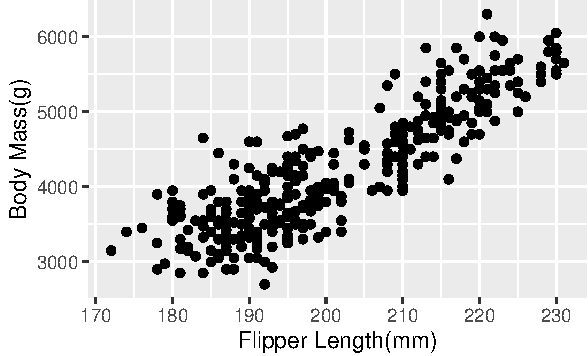
\includegraphics{R-Guide_files/figure-latex/scatter-plot-labs-1} \end{center}

So far we have only done stuff working within \texttt{aes}. Here is one
of the most common mistakes when working in \texttt{ggplot}, I still do
this!

\begin{Shaded}
\begin{Highlighting}[]
\FunctionTok{ggplot}\NormalTok{(penguins, }\FunctionTok{aes}\NormalTok{(}
  \AttributeTok{x =}\NormalTok{ flipper\_length\_mm, }\AttributeTok{y =}\NormalTok{ body\_mass\_g,}
  \AttributeTok{color =} \StringTok{"blue"}
\NormalTok{)) }\SpecialCharTok{+}
  \FunctionTok{geom\_point}\NormalTok{() }\SpecialCharTok{+}
  \FunctionTok{labs}\NormalTok{(}\AttributeTok{x =} \StringTok{"Flipper Length(mm)"}\NormalTok{, }\AttributeTok{y =} \StringTok{"Body Mass(g)"}\NormalTok{)}
\end{Highlighting}
\end{Shaded}

\begin{center}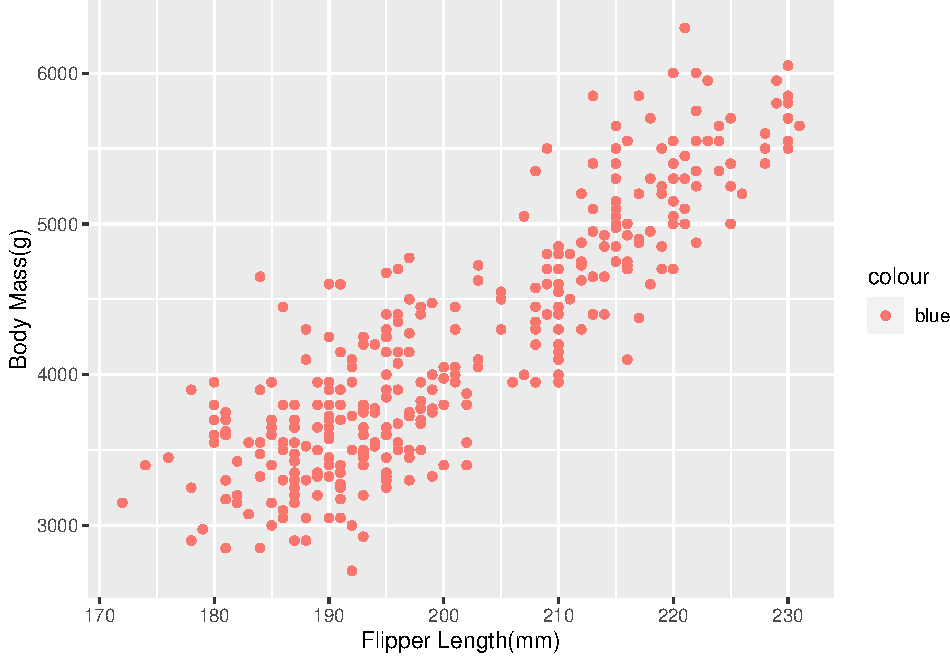
\includegraphics{R-Guide_files/figure-latex/mistake-easy-1} \end{center}

I wanted to change the color of the dots. However I did this in the
\texttt{aes()}. If you look back then, you will remember that
\texttt{aes} will look to put stuff in your plots based on
\textbf{columns} in your dataset. So to change the look of your plot,
you need to do it \textbf{outside} of \texttt{aes()}. So let's correct
that and then change the shape of the points.

\begin{Shaded}
\begin{Highlighting}[]
\FunctionTok{ggplot}\NormalTok{(penguins, }\FunctionTok{aes}\NormalTok{(}\AttributeTok{x =}\NormalTok{ flipper\_length\_mm, }\AttributeTok{y =}\NormalTok{ body\_mass\_g)) }\SpecialCharTok{+}
  \FunctionTok{geom\_point}\NormalTok{(}\AttributeTok{color =} \StringTok{"blue"}\NormalTok{, }\AttributeTok{shape =} \DecValTok{2}\NormalTok{) }\SpecialCharTok{+}
  \FunctionTok{labs}\NormalTok{(}\AttributeTok{x =} \StringTok{"Flipper Length(mm)"}\NormalTok{, }\AttributeTok{y =} \StringTok{"Body Mass(g)"}\NormalTok{)}
\end{Highlighting}
\end{Shaded}

\begin{center}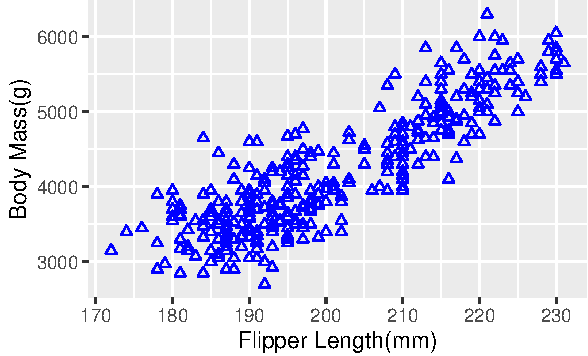
\includegraphics{R-Guide_files/figure-latex/real-changes-1} \end{center}

\hypertarget{subsetting-data-in-ggplot}{%
\subsection{Subsetting data in ggplot}\label{subsetting-data-in-ggplot}}

Let's say you want to look at a subset of the data. That is easy because
you can add in your friend \texttt{filter}.

\begin{Shaded}
\begin{Highlighting}[]
\FunctionTok{ggplot}\NormalTok{(penguins, }\FunctionTok{aes}\NormalTok{(}\AttributeTok{x =}\NormalTok{ flipper\_length\_mm, }\AttributeTok{y =}\NormalTok{ body\_mass\_g)) }\SpecialCharTok{+}
  \FunctionTok{geom\_point}\NormalTok{(}\AttributeTok{data =} \FunctionTok{filter}\NormalTok{(penguins, sex }\SpecialCharTok{==} \StringTok{"female"}\NormalTok{)) }\SpecialCharTok{+}
  \FunctionTok{labs}\NormalTok{(}\AttributeTok{x =} \StringTok{"Flipper Length(mm)"}\NormalTok{, }\AttributeTok{y =} \StringTok{"Body Mass(g)"}\NormalTok{)}
\end{Highlighting}
\end{Shaded}

\begin{center}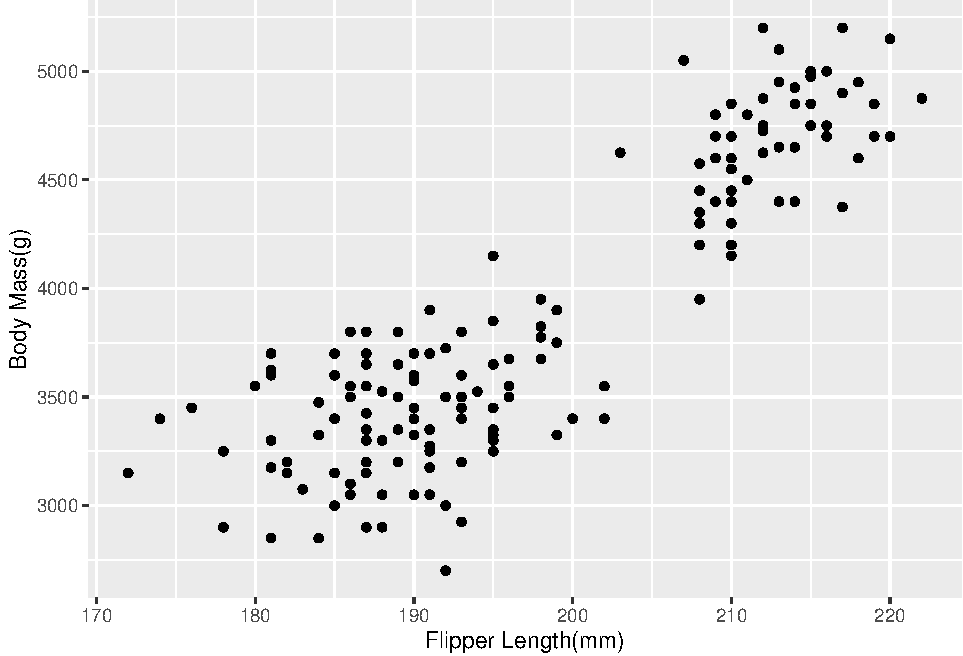
\includegraphics{R-Guide_files/figure-latex/female-plot-1} \end{center}

This also works.

\begin{Shaded}
\begin{Highlighting}[]
\NormalTok{penguins }\SpecialCharTok{\%\textgreater{}\%}
  \FunctionTok{filter}\NormalTok{(sex }\SpecialCharTok{==} \StringTok{"female"}\NormalTok{) }\SpecialCharTok{\%\textgreater{}\%}
  \FunctionTok{ggplot}\NormalTok{(}\FunctionTok{aes}\NormalTok{(}\AttributeTok{x =}\NormalTok{ flipper\_length\_mm, }\AttributeTok{y =}\NormalTok{ body\_mass\_g)) }\SpecialCharTok{+}
  \FunctionTok{geom\_point}\NormalTok{() }\SpecialCharTok{+}
  \FunctionTok{labs}\NormalTok{(}\AttributeTok{x =} \StringTok{"Flipper Length(mm)"}\NormalTok{, }\AttributeTok{y =} \StringTok{"Body Mass(g)"}\NormalTok{)}
\end{Highlighting}
\end{Shaded}

\begin{center}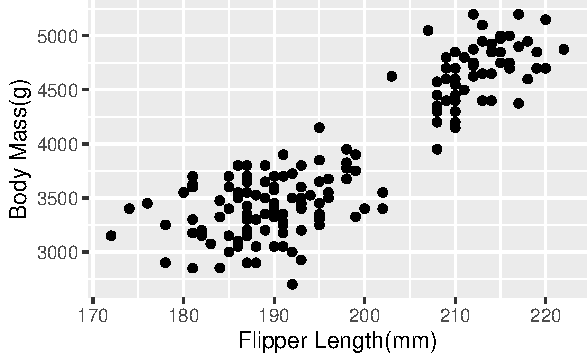
\includegraphics{R-Guide_files/figure-latex/female-plot-pipes-1} \end{center}

The difference is a matter of taste if we are being honest. I learned it
the first way, so I tend to do it that way. In the below plots let's
change the scale of the X and Y axis and then combine the two plots
using \texttt{patchwork}.

\begin{Shaded}
\begin{Highlighting}[]
\FunctionTok{library}\NormalTok{(scales)}
\NormalTok{fem\_plot }\OtherTok{\textless{}{-}}\NormalTok{ penguins }\SpecialCharTok{\%\textgreater{}\%}
  \FunctionTok{filter}\NormalTok{(sex }\SpecialCharTok{==} \StringTok{"female"}\NormalTok{) }\SpecialCharTok{\%\textgreater{}\%}
  \FunctionTok{ggplot}\NormalTok{(}\FunctionTok{aes}\NormalTok{(}\AttributeTok{x =}\NormalTok{ flipper\_length\_mm, }\AttributeTok{y =}\NormalTok{ body\_mass\_g)) }\SpecialCharTok{+}
  \FunctionTok{geom\_point}\NormalTok{() }\SpecialCharTok{+}
  \FunctionTok{labs}\NormalTok{(}\AttributeTok{x =} \StringTok{"Flipper Length(mm)"}\NormalTok{, }\AttributeTok{y =} \StringTok{"Body Mass(g)"}\NormalTok{, }\AttributeTok{title =} \StringTok{"Female"}\NormalTok{) }\SpecialCharTok{+}
  \FunctionTok{scale\_x\_continuous}\NormalTok{(}\AttributeTok{breaks =}\NormalTok{ scales}\SpecialCharTok{::}\FunctionTok{pretty\_breaks}\NormalTok{(}\AttributeTok{n =} \DecValTok{10}\NormalTok{))}


\NormalTok{fem\_plot}
\end{Highlighting}
\end{Shaded}

\begin{center}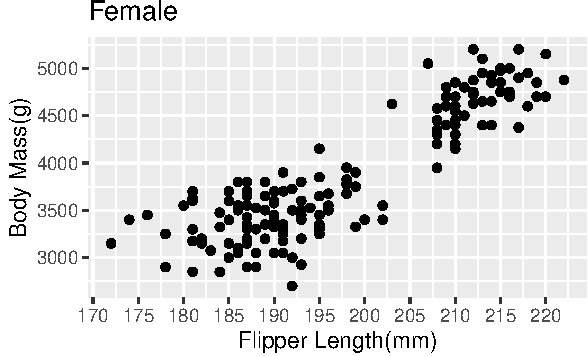
\includegraphics{R-Guide_files/figure-latex/female-plot-for-combo-1} \end{center}

\begin{Shaded}
\begin{Highlighting}[]
\NormalTok{male\_plot }\OtherTok{\textless{}{-}}\NormalTok{ penguins }\SpecialCharTok{\%\textgreater{}\%}
  \FunctionTok{filter}\NormalTok{(sex }\SpecialCharTok{==} \StringTok{"male"}\NormalTok{) }\SpecialCharTok{\%\textgreater{}\%}
  \FunctionTok{ggplot}\NormalTok{(}\FunctionTok{aes}\NormalTok{(}\AttributeTok{x =}\NormalTok{ flipper\_length\_mm, }\AttributeTok{y =}\NormalTok{ body\_mass\_g)) }\SpecialCharTok{+}
  \FunctionTok{geom\_point}\NormalTok{() }\SpecialCharTok{+}
  \FunctionTok{labs}\NormalTok{(}\AttributeTok{x =} \StringTok{"Flipper Length(mm)"}\NormalTok{, }\AttributeTok{y =} \StringTok{"Body Mass(g)"}\NormalTok{, }\AttributeTok{title =} \StringTok{"Male"}\NormalTok{) }\SpecialCharTok{+}
  \FunctionTok{scale\_x\_continuous}\NormalTok{(}\AttributeTok{breaks =}\NormalTok{ scales}\SpecialCharTok{::}\FunctionTok{pretty\_breaks}\NormalTok{(}\AttributeTok{n =} \DecValTok{10}\NormalTok{))}


\NormalTok{fem\_plot }\SpecialCharTok{/}\NormalTok{ male\_plot}
\end{Highlighting}
\end{Shaded}

\begin{center}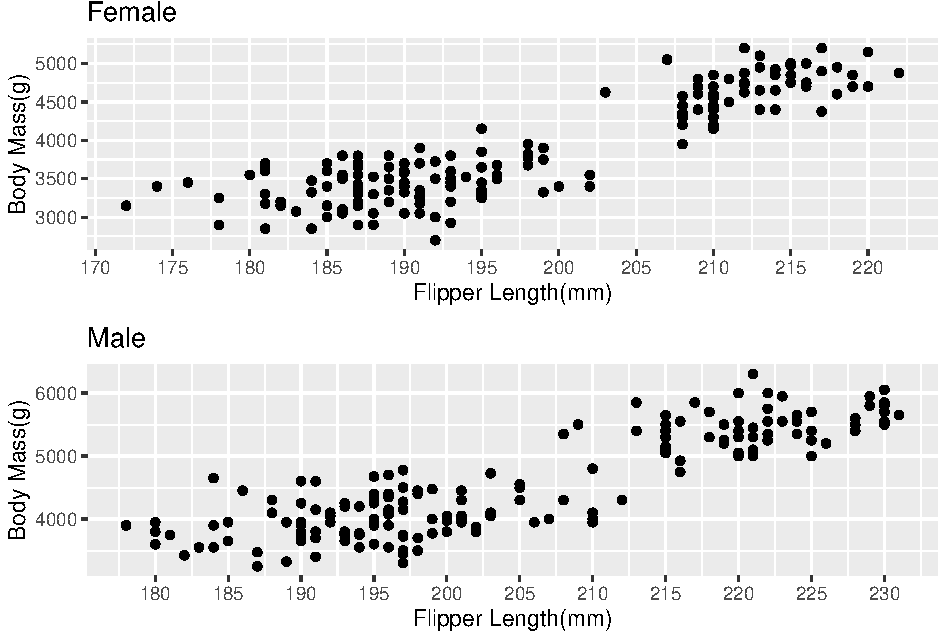
\includegraphics{R-Guide_files/figure-latex/female-plot-for-combo-2} \end{center}

\hypertarget{themes-in-ggplot}{%
\section{Themes in ggplot}\label{themes-in-ggplot}}

Themes are just ways to customize all the stuff that isn't data in your
plot. Themes make your graphs better looking and can make them stand
out.

The themes in \texttt{ggplot} get pretty intense very quickly. Lots of
people write their own themes, but this gets scary when you are first
learning ggplot, we will use \texttt{ggthemes} first, but as an example,
we will look at one I wrote for a class assignment that I use a lot.

\begin{verbatim}
theme_allen  = function(title_pos = "center", axis_title_pos = "left", slides = FALSE, has_subtitle = FALSE, base_size = 14, ...) {
  
  # Check if fonts were loaded. If not, load them
  if( !("Roboto Condensed" %in% sysfonts::font_families()) ) {
    sysfonts::font_add_google("Roboto Condensed", "Roboto Condensed")
    sysfonts::font_add_google("IBM Plex Sans", "IBM")
    showtext::showtext_auto()
  }
  
  title_hjust <- switch(title_pos, "center" = 0.5, "left" = 0)
  axis_title_hjust_y <- switch(axis_title_pos, "center" = 0.5, "left" = 1.0)
  axis_title_hjust_x <- switch(axis_title_pos, "center" = 0.5, "left" = 0.0)
  plot_bg = dplyr::if_else(slides, "#ECECEC", "transparent")
  plot_grid = dplyr::if_else(slides, "grey85", "grey92")
  title_margin = dplyr::if_else(has_subtitle, "4", "8")
  
  # Fix problems with axis ticks getting huge with large fonts
  if(base_size >= 20) {
    check_base_size = 20
  } else {
    check_base_size = base_size
  }
  
  ggplot2::theme_bw(
    base_size = check_base_size,
    base_family = "Roboto Condensed"
  ) +
    ggplot2::theme(
      ## Title and Subtitle --------------------------------------------------
      plot.title = ggplot2::element_text(
        # Font
        family = "Roboto Condensed", face = "bold", size = 1.285 * base_size,
        colour = "#454545",
        # Center title
        hjust = title_hjust,
        # Margins
        margin = ggplot2::margin(b = title_margin, unit = "pt")
      ),
      plot.subtitle = ggplot2::element_text(
        # Font
        family = "IBM", face = "italic", size = .86 * base_size,
        colour = "#454545",
        # Center subtitle
        hjust = title_hjust,
        # Margins
        margin = ggplot2::margin(b = 16, unit = "pt")
      ),
      plot.title.position = "plot",
      
      ## Caption -------------------------------------------------------------
      plot.caption = ggplot2::element_text(
        # Font
        size = 0.72 * base_size, colour = "#454545",
        # Right-align caption
        hjust = 1,
        # Margins
        margin = ggplot2::margin(t = 10)
      ),
      plot.caption.position = "plot",
      
      ## Axis ----------------------------------------------------------------
      # Axis title
      axis.title = ggplot2::element_text(
        # Font
        size = .86 * base_size, colour = "#454545", face = "italic"
      ),
      # Axis Title x/y
      axis.title.y = ggplot2::element_text(
        # Right-align y axis title
        hjust = axis_title_hjust_y,
        # Margins
        margin = ggplot2::margin(r = 5)
      ),
      axis.title.x = ggplot2::element_text(
        # Left-align x axis title
        hjust = axis_title_hjust_x,
        # Margins
        margin = ggplot2::margin(t = 5)
      ),
      # Axis labels
      axis.text = ggplot2::element_text(
        # Font
        size = .72 * base_size, colour = "#212121"
      ),
      # Axis Lines
      axis.line = ggplot2::element_line(
        colour = "grey40"
      ),
      panel.grid = ggplot2::element_line(
        colour = plot_grid
      ),
      
      
      ## Legend -------------------------------------------------------------
      # Legend title
      legend.title = ggplot2::element_text(
        # Font
        size = .86 * base_size, colour = "#454545"
      ),
      # Legend labels
      legend.text = ggplot2::element_text(
        # Font
        size = .72 * base_size, colour = "#454545"
      ),
      legend.background = ggplot2::element_rect(
        # No Background Colour
        fill = "transparent", colour = NA
      ),
      legend.key = ggplot2::element_rect(
        # No Background Colour
        fill = "transparent", colour = NA
      ),
      
      
      ## Facet Wrap ----------------------------------------------------------
      strip.text = ggplot2::element_text(
        # Font
        size = .86 * base_size, colour = "#454545",
        # Margin
        margin = ggplot2::margin(t= 10, b= 10)
      ),
      strip.background = ggplot2::element_rect(
        # No Background Colour
        fill = "transparent", colour = NA
      ),
      
      ## Panel ---------------------------------------------------------------
      panel.background = ggplot2::element_rect(
        # No Background Colour
        fill = plot_bg, colour = NA
      ),
      panel.border = ggplot2::element_rect(
        # No Background Colour
        colour = NA
      ),
      panel.spacing = grid::unit(8, "points"),
      ## Plot ----------------------------------------------------------------
      plot.background = ggplot2::element_rect(
        # No Background Colour
        fill = plot_bg, colour = NA
      ),
      plot.margin = ggplot2::margin(16, 16, 16, 16, unit = "pt")
    ) +
    ## Additional options passed by user ---------------------------------------
  ggplot2::theme(
    ...
  )}


\end{verbatim}

This is what this looks like in action.

\begin{Shaded}
\begin{Highlighting}[]
\NormalTok{color1 }\OtherTok{\textless{}{-}} \FunctionTok{get\_pal}\NormalTok{(}\StringTok{"Kaka"}\NormalTok{)}

\FunctionTok{ggplot}\NormalTok{(}\AttributeTok{data =}\NormalTok{ penguins, }\FunctionTok{aes}\NormalTok{(}
  \AttributeTok{x =}\NormalTok{ flipper\_length\_mm, }\AttributeTok{y =}\NormalTok{ body\_mass\_g, }\AttributeTok{color =}\NormalTok{ species,}
  \AttributeTok{shape =}\NormalTok{ species}
\NormalTok{)) }\SpecialCharTok{+}
  \FunctionTok{geom\_point}\NormalTok{(}\AttributeTok{position =} \FunctionTok{position\_jitter}\NormalTok{(}\AttributeTok{width =} \DecValTok{0}\NormalTok{, }\AttributeTok{height =} \FloatTok{0.25}\NormalTok{, }\AttributeTok{seed =} \DecValTok{1234}\NormalTok{)) }\SpecialCharTok{+}
  \FunctionTok{geom\_smooth}\NormalTok{(}\AttributeTok{method =} \StringTok{"lm"}\NormalTok{, }\AttributeTok{se =} \ConstantTok{FALSE}\NormalTok{) }\SpecialCharTok{+}
  \FunctionTok{labs}\NormalTok{(}\AttributeTok{x =} \StringTok{"Flipper Length(mm)"}\NormalTok{, }\AttributeTok{y =} \StringTok{"Body Mass(g)"}\NormalTok{, }\AttributeTok{fill =} \StringTok{"Species of Penguins"}\NormalTok{) }\SpecialCharTok{+}
  \FunctionTok{scale\_color\_manual}\NormalTok{(}\AttributeTok{values =}\NormalTok{ color1) }\SpecialCharTok{+}
  \FunctionTok{scale\_x\_continuous}\NormalTok{(}\AttributeTok{breaks =}\NormalTok{ scales}\SpecialCharTok{::}\FunctionTok{pretty\_breaks}\NormalTok{(}\AttributeTok{n =} \DecValTok{10}\NormalTok{)) }\SpecialCharTok{+}
  \FunctionTok{scale\_y\_continuous}\NormalTok{(}\AttributeTok{breaks =}\NormalTok{ scales}\SpecialCharTok{::}\FunctionTok{pretty\_breaks}\NormalTok{(}\AttributeTok{n =} \DecValTok{10}\NormalTok{)) }\SpecialCharTok{+}
  \FunctionTok{theme\_allen}\NormalTok{()}
\end{Highlighting}
\end{Shaded}

\begin{center}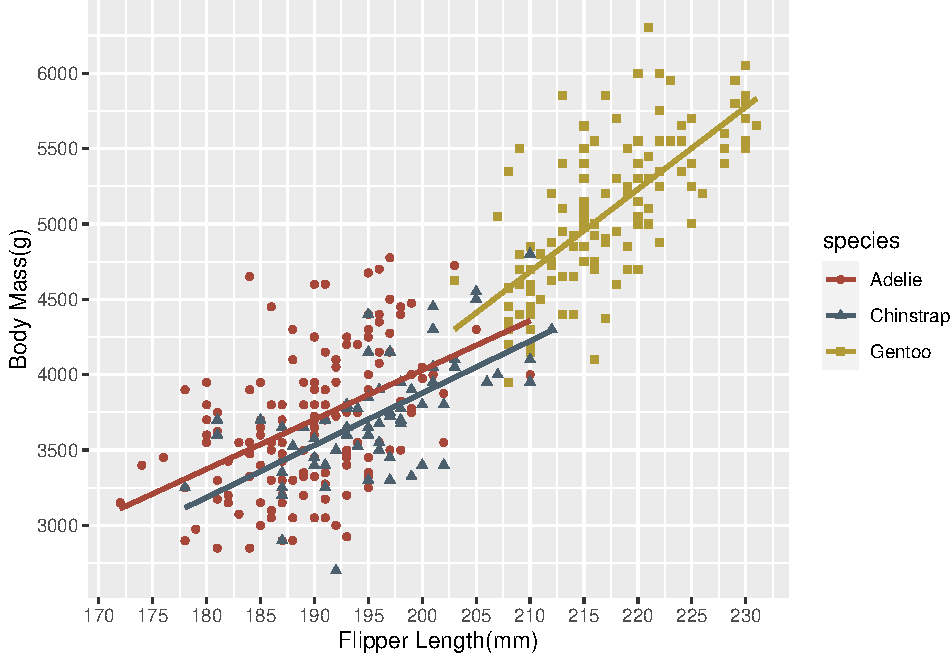
\includegraphics{R-Guide_files/figure-latex/multiplot-1} \end{center}

\hypertarget{what-else-can-i-do-in-ggplot}{%
\subsection{\texorpdfstring{What else can I do in
\texttt{ggplot}?}{What else can I do in ggplot?}}\label{what-else-can-i-do-in-ggplot}}

\texttt{ggplot} has a ton of flexibility that you can take courses on,
so I will provide some examples of graphics I have made in
\texttt{ggplot}.

\begin{Shaded}
\begin{Highlighting}[]
\FunctionTok{theme\_set}\NormalTok{(}
  \FunctionTok{theme\_allen}\NormalTok{()}
\NormalTok{)}


\FunctionTok{ggplot}\NormalTok{(penguins, }\FunctionTok{aes}\NormalTok{(}\AttributeTok{x =}\NormalTok{ flipper\_length\_mm, }\AttributeTok{y =}\NormalTok{ body\_mass\_g)) }\SpecialCharTok{+}
  \FunctionTok{geom\_point}\NormalTok{(}\AttributeTok{data =} \FunctionTok{filter}\NormalTok{(penguins, sex }\SpecialCharTok{==} \StringTok{"female"}\NormalTok{)) }\SpecialCharTok{+}
  \FunctionTok{labs}\NormalTok{(}\AttributeTok{x =} \StringTok{"Flipper Length(mm)"}\NormalTok{, }\AttributeTok{y =} \StringTok{"Body Mass(g)"}\NormalTok{)}
\end{Highlighting}
\end{Shaded}

\begin{center}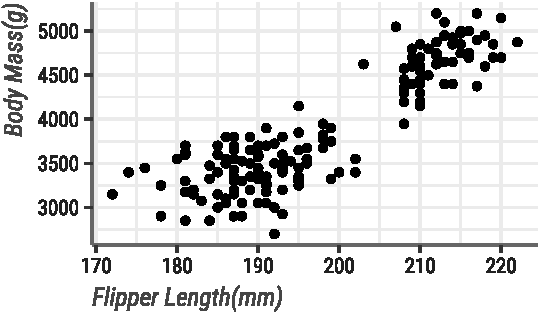
\includegraphics{R-Guide_files/figure-latex/penguins-example-with-fonts-1} \end{center}

You can make maps in \texttt{ggplot}.

\begin{center}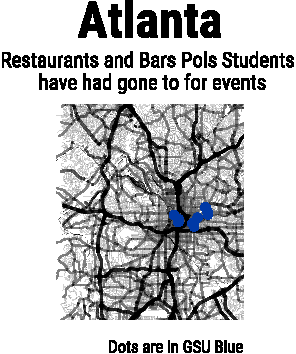
\includegraphics{R-Guide_files/figure-latex/map-1} \end{center}

\hypertarget{other-useful-stuff}{%
\section{Other Useful Stuff}\label{other-useful-stuff}}

So for this class, you will have to make some tables, and there are a
lot of mistakes you can make when you are trying to format tables
manually. But, just as important, it is tedious and annoying, so why
would you waste time doing that if there is an automated way to do that?
We have already loaded in our friend \texttt{modelsummary}, and since
this is a \texttt{Rmarkdown} document, our friend \texttt{kable} is also
loaded. So let's see some examples of how to do this. Let's create a
fake dataset about the effect of going to math camp on GRE scores.

\begin{Shaded}
\begin{Highlighting}[]
\NormalTok{pacman}\SpecialCharTok{::}\FunctionTok{p\_load}\NormalTok{(}\StringTok{"kableExtra"}\NormalTok{, }\StringTok{"truncnorm"}\NormalTok{, }\StringTok{"broom"}\NormalTok{)}

\NormalTok{n\_people }\OtherTok{\textless{}{-}} \DecValTok{2500}

\NormalTok{grade\_data }\OtherTok{\textless{}{-}} \FunctionTok{tibble}\NormalTok{(}
  \AttributeTok{id =} \DecValTok{1}\SpecialCharTok{:}\NormalTok{n\_people,}
  \AttributeTok{gpa =} \FunctionTok{rtruncnorm}\NormalTok{(n\_people,}
    \AttributeTok{mean =} \FloatTok{3.5}\NormalTok{, }\AttributeTok{sd =} \FloatTok{1.0}\NormalTok{,}
    \AttributeTok{a =} \FloatTok{1.5}\NormalTok{, }\AttributeTok{b =} \FloatTok{4.0}
\NormalTok{  )}
\NormalTok{) }\SpecialCharTok{\%\textgreater{}\%}
  \FunctionTok{mutate}\NormalTok{(}
    \AttributeTok{gpa =} \FunctionTok{round}\NormalTok{(gpa, }\DecValTok{2}\NormalTok{),}
    \AttributeTok{gre\_base =} \FunctionTok{rbeta}\NormalTok{(n\_people, }\AttributeTok{shape1 =} \DecValTok{3}\NormalTok{, }\AttributeTok{shape2 =} \DecValTok{16}\NormalTok{),}
    \AttributeTok{gre\_effect =} \FloatTok{10.1} \SpecialCharTok{*}\NormalTok{ gpa,}
    \AttributeTok{gre =}\NormalTok{ gre\_base }\SpecialCharTok{+}\NormalTok{ gre\_effect }\SpecialCharTok{+} \FunctionTok{rnorm}\NormalTok{(n\_people, }\AttributeTok{mean =} \DecValTok{150}\NormalTok{, }\AttributeTok{sd =} \FloatTok{3.5}\NormalTok{),}
    \AttributeTok{gre =} \FunctionTok{round}\NormalTok{(gre, }\DecValTok{0}\NormalTok{),}
    \AttributeTok{math\_score =}\NormalTok{ (gre }\SpecialCharTok{*} \SpecialCharTok{{-}}\FloatTok{10.0}\NormalTok{) }\SpecialCharTok{+}\NormalTok{ (gpa }\SpecialCharTok{*} \SpecialCharTok{{-}}\FloatTok{2.0}\NormalTok{) }\SpecialCharTok{+} \FunctionTok{rnorm}\NormalTok{(n\_people,}
      \AttributeTok{mean =} \DecValTok{0}\NormalTok{,}
      \AttributeTok{sd =} \DecValTok{3}
\NormalTok{    ),}
    \AttributeTok{math\_probability =} \FunctionTok{rescale}\NormalTok{(math\_score, }\AttributeTok{to =} \FunctionTok{c}\NormalTok{(}\FloatTok{0.05}\NormalTok{, }\FloatTok{0.95}\NormalTok{)),}
    \AttributeTok{math\_camp\_num =} \FunctionTok{rbinom}\NormalTok{(n\_people, }\DecValTok{1}\NormalTok{, math\_probability),}
    \AttributeTok{math\_camp =} \FunctionTok{ifelse}\NormalTok{(math\_camp\_num }\SpecialCharTok{==} \DecValTok{1}\NormalTok{, }\ConstantTok{TRUE}\NormalTok{, }\ConstantTok{FALSE}\NormalTok{)}
\NormalTok{  ) }\SpecialCharTok{\%\textgreater{}\%}
  \FunctionTok{mutate}\NormalTok{(}
    \AttributeTok{grade\_base =} \FunctionTok{rbeta}\NormalTok{(n\_people, }\AttributeTok{shape1 =} \DecValTok{4}\NormalTok{, }\AttributeTok{shape2 =} \DecValTok{5}\NormalTok{) }\SpecialCharTok{*} \DecValTok{100}\NormalTok{,}
    \AttributeTok{grade\_effect =}\NormalTok{ (}\DecValTok{15} \SpecialCharTok{*}\NormalTok{ gpa) }\SpecialCharTok{+}\NormalTok{ (}\DecValTok{2} \SpecialCharTok{*}\NormalTok{ gre) }\SpecialCharTok{+}\NormalTok{ (}\DecValTok{10} \SpecialCharTok{*}\NormalTok{ math\_camp),}
    \AttributeTok{final\_grade =}\NormalTok{ grade\_base }\SpecialCharTok{+}\NormalTok{ grade\_effect }\SpecialCharTok{+} \FunctionTok{rnorm}\NormalTok{(n\_people, }\DecValTok{0}\NormalTok{, }\AttributeTok{sd =} \DecValTok{2}\NormalTok{),}
    \AttributeTok{final\_grade =} \FunctionTok{rescale}\NormalTok{(final\_grade, }\AttributeTok{to =} \FunctionTok{c}\NormalTok{(}\DecValTok{0}\NormalTok{, }\DecValTok{100}\NormalTok{)),}
    \AttributeTok{final\_grade =} \FunctionTok{round}\NormalTok{(final\_grade, }\DecValTok{1}\NormalTok{)}
\NormalTok{  )}
\end{Highlighting}
\end{Shaded}

So here are a bunch of models that you should not worry about. We use a
mixture of base \texttt{R} functions and \texttt{tidyverse} friends.

\begin{Shaded}
\begin{Highlighting}[]
\CommentTok{\# For lm we need to feed it the data argument}
\NormalTok{naive\_model }\OtherTok{\textless{}{-}} \FunctionTok{lm}\NormalTok{(final\_grade }\SpecialCharTok{\textasciitilde{}}\NormalTok{ math\_camp, }\AttributeTok{data =}\NormalTok{ grade\_data)}
\FunctionTok{tidy}\NormalTok{(naive\_model)}


\NormalTok{adjusted\_mod }\OtherTok{\textless{}{-}} \FunctionTok{lm}\NormalTok{(final\_grade }\SpecialCharTok{\textasciitilde{}}\NormalTok{ math\_camp }\SpecialCharTok{+}\NormalTok{ gre }\SpecialCharTok{+}\NormalTok{ gpa, }\AttributeTok{data =}\NormalTok{ grade\_data)}
\FunctionTok{tidy}\NormalTok{(adjusted\_mod)}



\NormalTok{prop\_model }\OtherTok{\textless{}{-}} \FunctionTok{glm}\NormalTok{(math\_camp }\SpecialCharTok{\textasciitilde{}}\NormalTok{ gre }\SpecialCharTok{+}\NormalTok{ gpa,}
  \AttributeTok{family =} \FunctionTok{binomial}\NormalTok{(}\AttributeTok{link =} \StringTok{"logit"}\NormalTok{),}
  \AttributeTok{data =}\NormalTok{ grade\_data}
\NormalTok{)}

\NormalTok{camp\_probabilities }\OtherTok{\textless{}{-}} \FunctionTok{augment\_columns}\NormalTok{(prop\_model,}
\NormalTok{  grade\_data,}
  \AttributeTok{type.predict =} \StringTok{"response"}
\NormalTok{) }\SpecialCharTok{\%\textgreater{}\%}
  \FunctionTok{rename}\NormalTok{(}\AttributeTok{propensity =}\NormalTok{ .fitted)}


\NormalTok{camp\_weights }\OtherTok{\textless{}{-}}\NormalTok{ camp\_probabilities }\SpecialCharTok{\%\textgreater{}\%}
  \DocumentationTok{\#\#\# To ensure that R doesn\textquotesingle{}t do something weird with precedence lets wrap that}
  \DocumentationTok{\#\#\# in parenthesis}
  \FunctionTok{mutate}\NormalTok{(}\AttributeTok{ipw =}\NormalTok{ (math\_camp }\SpecialCharTok{/}\NormalTok{ propensity) }\SpecialCharTok{+}\NormalTok{ (}\DecValTok{1} \SpecialCharTok{{-}}\NormalTok{ math\_camp) }\SpecialCharTok{/}\NormalTok{ (}\DecValTok{1} \SpecialCharTok{{-}}\NormalTok{ propensity))}

\NormalTok{ipw\_model }\OtherTok{\textless{}{-}} \FunctionTok{lm}\NormalTok{(final\_grade }\SpecialCharTok{\textasciitilde{}}\NormalTok{ math\_camp, }\AttributeTok{weights =}\NormalTok{ ipw, }\AttributeTok{data =}\NormalTok{ camp\_weights)}
\FunctionTok{tidy}\NormalTok{(ipw\_model)}
\end{Highlighting}
\end{Shaded}

So we have a bunch of statsy stuff we want to put in a table so let's do
that!

\begin{Shaded}
\begin{Highlighting}[]
\FunctionTok{modelsummary}\NormalTok{(}\FunctionTok{list}\NormalTok{(}
  \StringTok{"Naive"} \OtherTok{=}\NormalTok{ naive\_model, }\StringTok{"Confounders"} \OtherTok{=}\NormalTok{ adjusted\_mod,}
  \StringTok{"IPW"} \OtherTok{=}\NormalTok{ ipw\_model}
\NormalTok{),}
\AttributeTok{stars =} \ConstantTok{TRUE}\NormalTok{,}
\AttributeTok{output =} \StringTok{"kableExtra"}\NormalTok{,}
\AttributeTok{gof\_omit =} \StringTok{"IC|Log|F|Adj"}\NormalTok{,}
\AttributeTok{coef\_map =} \FunctionTok{c}\NormalTok{(}
  \StringTok{"math\_campTRUE"} \OtherTok{=} \StringTok{"Math Camp"}\NormalTok{, }\StringTok{"gre"} \OtherTok{=} \StringTok{"GRE"}\NormalTok{,}
  \StringTok{"gpa"} \OtherTok{=} \StringTok{"GPA"}\NormalTok{, }\StringTok{"(Intercept)"} \OtherTok{=} \StringTok{"Constant"}
\NormalTok{),}
\AttributeTok{title =} \StringTok{"Effect of Math Camp on Final Grade }\SpecialCharTok{\textbackslash{}\textbackslash{}}\StringTok{label\{tab:table1\}"}
\NormalTok{) }\SpecialCharTok{\%\textgreater{}\%}
  \FunctionTok{kable\_styling}\NormalTok{(}\AttributeTok{latex\_options =} \StringTok{"HOLD\_position"}\NormalTok{)}
\end{Highlighting}
\end{Shaded}

\begin{table}[H]

\caption{\label{tab:table-making}Effect of Math Camp on Final Grade \label{tab:table1}}
\centering
\begin{tabular}[t]{lccc}
\toprule
  & Naive & Confounders & IPW\\
\midrule
Math Camp & \num{-2.950}*** & \num{6.478}*** & \num{6.263}***\\
 & (\num{0.657}) & (\num{0.425}) & (\num{0.674})\\
GRE &  & \num{1.292}*** & \\
 &  & (\num{0.058}) & \\
GPA &  & \num{8.666}*** & \\
 &  & (\num{0.668}) & \\
Constant & \num{51.095}*** & \num{-213.396}*** & \num{47.091}***\\
 & (\num{0.437}) & (\num{8.830}) & (\num{0.476})\\
\midrule
Num.Obs. & \num{2500} & \num{2500} & \num{2500}\\
R2 & \num{0.008} & \num{0.634} & \num{0.033}\\
RMSE & \num{16.32} & \num{9.92} & \num{23.79}\\
\bottomrule
\multicolumn{4}{l}{\rule{0pt}{1em}+ p $<$ 0.1, * p $<$ 0.05, ** p $<$ 0.01, *** p $<$ 0.001}\\
\end{tabular}
\end{table}

Now we have a pretty table of stats results. Don't worry too much about
the statsy stuff that we did in this case because that is a whole course
that somebody far more qualified than I should be teaching you.

\begin{Shaded}
\begin{Highlighting}[]
\FunctionTok{datasummary}\NormalTok{(gpa }\SpecialCharTok{\textasciitilde{}}\NormalTok{ Mean, }\AttributeTok{data =}\NormalTok{ grade\_data)}
\end{Highlighting}
\end{Shaded}

\begin{table}
\centering
\begin{tabular}[t]{lr}
\toprule
  & Mean\\
\midrule
gpa & \num{3.06}\\
\bottomrule
\end{tabular}
\end{table}

Doing individual tables for each variable will be annoying for you and
the reader, so what if we wanted to add more variables and more stats?
You can slowly build this up, but looking at the help documentation will
be your best bet!

\begin{Shaded}
\begin{Highlighting}[]
\FunctionTok{datasummary}\NormalTok{(gpa }\SpecialCharTok{+}\NormalTok{ gre }\SpecialCharTok{\textasciitilde{}}\NormalTok{ Mean }\SpecialCharTok{+}\NormalTok{ SD,}
  \AttributeTok{data =}\NormalTok{ grade\_data}
\NormalTok{)}
\end{Highlighting}
\end{Shaded}

\begin{table}
\centering
\begin{tabular}[t]{lrr}
\toprule
  & Mean & SD\\
\midrule
gpa & \num{3.06} & \num{0.60}\\
gre & \num{181.04} & \num{6.99}\\
\bottomrule
\end{tabular}
\end{table}

\hypertarget{resources}{%
\section{Resources}\label{resources}}

\hypertarget{getting-started-1}{%
\subsection{Getting Started}\label{getting-started-1}}

\begin{itemize}
\item
  \href{https://r4ds.had.co.nz/index.html}{R4Ds} is perhaps the ultimate
  starter book for the \texttt{tidyverse} written by the authors of the
  \texttt{tidyverse} and should be your first stop.
\item
  \href{https://rstudio-education.github.io/hopr/}{Hands on Programing}
\item
  \href{https://cran.r-project.org/doc/manuals/R-intro.pdf}{R Core
  Manual}
\item
  \href{http://adv-r.had.co.nz/}{Advanced Stuff}
\end{itemize}

\hypertarget{rmarkdown}{%
\subsection{Rmarkdown}\label{rmarkdown}}

\href{https://bookdown.org/yihui/rmarkdown/}{It really is definitive}

\hypertarget{ggplot}{%
\subsection{ggplot}\label{ggplot}}

Perhaps \texttt{R\textquotesingle{}s} most beloved and used package in
the \texttt{tidyverse}. I will say that I never really read anything on
\texttt{ggplot} and tend to go full steam ahead into doing stuff. But
these are the resources I use most often.

\begin{itemize}
\tightlist
\item
  \href{https://r-graphics.org/}{Cookbook}
\item
  \href{https://ggplot2-book.org/index.html}{All about ggplot}
\item
  \href{https://datavizs21.classes.andrewheiss.com/}{Free class}
\item
  \href{https://socviz.co/}{V influential book in the social sciences}
\end{itemize}

\hypertarget{misc}{%
\subsection{misc}\label{misc}}

Working with text data has a lot of idiosyncrasies and takes a lot of
wrangling. I switched from Word to LaTeX a few years ago but never liked
beamer presentations. So I use \texttt{xaringan} to create all my
slides.

\begin{itemize}
\tightlist
\item
  \href{https://www.tidytextmining.com/index.html}{tidytext}
\item
  \href{https://apreshill.github.io/data-vis-labs-2018/slides.html}{xaringan
  primer}
\end{itemize}



\end{document}
